\documentclass[12pt]{article}

%packages
%\usepackage{latexsym}
\usepackage{graphicx}
\usepackage{color}
\usepackage{amsmath}
\usepackage{dsfont}
\usepackage{placeins}
\usepackage{amssymb}
\usepackage{wasysym}
\usepackage{abstract}
\usepackage{hyperref}
\usepackage{etoolbox}
\usepackage{datetime}
\usepackage{xcolor}
\usepackage{alphalph}
\settimeformat{ampmtime}

%\usepackage{pstricks,pst-node,pst-tree}

%\usepackage{algpseudocode}
%\usepackage{amsthm}
%\usepackage{hyperref}
%\usepackage{mathrsfs}
%\usepackage{amsfonts}
%\usepackage{bbding}
%\usepackage{listings}
%\usepackage{appendix}
\usepackage[margin=1in]{geometry}
%\geometry{papersize={8.5in,11in},total={6.5in,9in}}
%\usepackage{cancel}
%\usepackage{algorithmic, algorithm}

\makeatletter
\def\maxwidth{ %
  \ifdim\Gin@nat@width>\linewidth
    \linewidth
  \else
    \Gin@nat@width
  \fi
}
\makeatother

\definecolor{fgcolor}{rgb}{0.345, 0.345, 0.345}
\newcommand{\hlnum}[1]{\textcolor[rgb]{0.686,0.059,0.569}{#1}}%
\newcommand{\hlstr}[1]{\textcolor[rgb]{0.192,0.494,0.8}{#1}}%
\newcommand{\hlcom}[1]{\textcolor[rgb]{0.678,0.584,0.686}{\textit{#1}}}%
\newcommand{\hlopt}[1]{\textcolor[rgb]{0,0,0}{#1}}%
\newcommand{\hlstd}[1]{\textcolor[rgb]{0.345,0.345,0.345}{#1}}%
\newcommand{\hlkwa}[1]{\textcolor[rgb]{0.161,0.373,0.58}{\textbf{#1}}}%
\newcommand{\hlkwb}[1]{\textcolor[rgb]{0.69,0.353,0.396}{#1}}%
\newcommand{\hlkwc}[1]{\textcolor[rgb]{0.333,0.667,0.333}{#1}}%
\newcommand{\hlkwd}[1]{\textcolor[rgb]{0.737,0.353,0.396}{\textbf{#1}}}%

\usepackage{framed}
\makeatletter
\newenvironment{kframe}{%
 \def\at@end@of@kframe{}%
 \ifinner\ifhmode%
  \def\at@end@of@kframe{\end{minipage}}%
  \begin{minipage}{\columnwidth}%
 \fi\fi%
 \def\FrameCommand##1{\hskip\@totalleftmargin \hskip-\fboxsep
 \colorbox{shadecolor}{##1}\hskip-\fboxsep
     % There is no \\@totalrightmargin, so:
     \hskip-\linewidth \hskip-\@totalleftmargin \hskip\columnwidth}%
 \MakeFramed {\advance\hsize-\width
   \@totalleftmargin\z@ \linewidth\hsize
   \@setminipage}}%
 {\par\unskip\endMakeFramed%
 \at@end@of@kframe}
\makeatother

\definecolor{shadecolor}{rgb}{.77, .77, .77}
\definecolor{messagecolor}{rgb}{0, 0, 0}
\definecolor{warningcolor}{rgb}{1, 0, 1}
\definecolor{errorcolor}{rgb}{1, 0, 0}
\newenvironment{knitrout}{}{} % an empty environment to be redefined in TeX

\usepackage{alltt}
\usepackage[T1]{fontenc}

\newcommand{\qu}[1]{``#1''}
\newcounter{probnum}
\setcounter{probnum}{1}

%create definition to allow local margin changes
\def\changemargin#1#2{\list{}{\rightmargin#2\leftmargin#1}\item[]}
\let\endchangemargin=\endlist 

%allow equations to span multiple pages
\allowdisplaybreaks

%define colors and color typesetting conveniences
\definecolor{gray}{rgb}{0.5,0.5,0.5}
\definecolor{black}{rgb}{0,0,0}
\definecolor{white}{rgb}{1,1,1}
\definecolor{blue}{rgb}{0.5,0.5,1}
\newcommand{\inblue}[1]{\color{blue}#1 \color{black}}
\definecolor{green}{rgb}{0.133,0.545,0.133}
\newcommand{\ingreen}[1]{\color{green}#1 \color{black}}
\definecolor{yellow}{rgb}{1,1,0}
\newcommand{\inyellow}[1]{\color{yellow}#1 \color{black}}
\definecolor{orange}{rgb}{0.9,0.649,0}
\newcommand{\inorange}[1]{\color{orange}#1 \color{black}}
\definecolor{red}{rgb}{1,0.133,0.133}
\newcommand{\inred}[1]{\color{red}#1 \color{black}}
\definecolor{purple}{rgb}{0.58,0,0.827}
\newcommand{\inpurple}[1]{\color{purple}#1 \color{black}}
\definecolor{backgcode}{rgb}{0.97,0.97,0.8}
\definecolor{Brown}{cmyk}{0,0.81,1,0.60}
\definecolor{OliveGreen}{cmyk}{0.64,0,0.95,0.40}
\definecolor{CadetBlue}{cmyk}{0.62,0.57,0.23,0}

%define new math operators
\DeclareMathOperator*{\argmax}{arg\,max~}
\DeclareMathOperator*{\argmin}{arg\,min~}
\DeclareMathOperator*{\argsup}{arg\,sup~}
\DeclareMathOperator*{\arginf}{arg\,inf~}
\DeclareMathOperator*{\convolution}{\text{\Huge{$\ast$}}}
\newcommand{\infconv}[2]{\convolution^\infty_{#1 = 1} #2}
%true functions

%%%% GENERAL SHORTCUTS

%shortcuts for pure typesetting conveniences
\newcommand{\bv}[1]{\boldsymbol{#1}}

%shortcuts for compound constants
\newcommand{\BetaDistrConst}{\dfrac{\Gamma(\alpha + \beta)}{\Gamma(\alpha)\Gamma(\beta)}}
\newcommand{\NormDistrConst}{\dfrac{1}{\sqrt{2\pi\sigma^2}}}

%shortcuts for conventional symbols
\newcommand{\tsq}{\tau^2}
\newcommand{\tsqh}{\hat{\tau}^2}
\newcommand{\sigsq}{\sigma^2}
\newcommand{\sigsqsq}{\parens{\sigma^2}^2}
\newcommand{\sigsqovern}{\dfrac{\sigsq}{n}}
\newcommand{\tausq}{\tau^2}
\newcommand{\tausqalpha}{\tau^2_\alpha}
\newcommand{\tausqbeta}{\tau^2_\beta}
\newcommand{\tausqsigma}{\tau^2_\sigma}
\newcommand{\betasq}{\beta^2}
\newcommand{\sigsqvec}{\bv{\sigma}^2}
\newcommand{\sigsqhat}{\hat{\sigma}^2}
\newcommand{\sigsqhatmlebayes}{\sigsqhat_{\text{Bayes, MLE}}}
\newcommand{\sigsqhatmle}[1]{\sigsqhat_{#1, \text{MLE}}}
\newcommand{\bSigma}{\bv{\Sigma}}
\newcommand{\bSigmainv}{\bSigma^{-1}}
\newcommand{\thetavec}{\bv{\theta}}
\newcommand{\thetahat}{\hat{\theta}}
\newcommand{\thetahatmle}{\hat{\theta}_{\mathrm{MLE}}}
\newcommand{\thetavechatmle}{\hat{\thetavec}_{\mathrm{MLE}}}
\newcommand{\muhat}{\hat{\mu}}
\newcommand{\musq}{\mu^2}
\newcommand{\muvec}{\bv{\mu}}
\newcommand{\muhatmle}{\muhat_{\text{MLE}}}
\newcommand{\lambdahat}{\hat{\lambda}}
\newcommand{\lambdahatmle}{\lambdahat_{\text{MLE}}}
\newcommand{\etavec}{\bv{\eta}}
\newcommand{\alphavec}{\bv{\alpha}}
\newcommand{\minimaxdec}{\delta^*_{\mathrm{mm}}}
\newcommand{\ybar}{\bar{y}}
\newcommand{\xbar}{\bar{x}}
\newcommand{\Xbar}{\bar{X}}
\newcommand{\phat}{\hat{p}}
\newcommand{\Phat}{\hat{P}}
\newcommand{\Zbar}{\bar{Z}}
\newcommand{\iid}{~{\buildrel iid \over \sim}~}
\newcommand{\inddist}{~{\buildrel ind \over \sim}~}
\newcommand{\approxdist}{~{\buildrel approx \over \sim}~}
\newcommand{\equalsindist}{~{\buildrel d \over =}~}
\newcommand{\loglik}[1]{\ell\parens{#1}}
\newcommand{\thetahatkminone}{\thetahat^{(k-1)}}
\newcommand{\thetahatkplusone}{\thetahat^{(k+1)}}
\newcommand{\thetahatk}{\thetahat^{(k)}}
\newcommand{\half}{\frac{1}{2}}
\newcommand{\third}{\frac{1}{3}}
\newcommand{\twothirds}{\frac{2}{3}}
\newcommand{\fourth}{\frac{1}{4}}
\newcommand{\fifth}{\frac{1}{5}}
\newcommand{\sixth}{\frac{1}{6}}

%shortcuts for vector and matrix notation
\newcommand{\A}{\bv{A}}
\newcommand{\At}{\A^T}
\newcommand{\Ainv}{\inverse{\A}}
\newcommand{\B}{\bv{B}}
\newcommand{\K}{\bv{K}}
\newcommand{\Kt}{\K^T}
\newcommand{\Kinv}{\inverse{K}}
\newcommand{\Kinvt}{(\Kinv)^T}
\newcommand{\M}{\bv{M}}
\newcommand{\Bt}{\B^T}
\newcommand{\Q}{\bv{Q}}
\newcommand{\Qt}{\Q^T}
\newcommand{\R}{\bv{R}}
\newcommand{\Rt}{\R^T}
\newcommand{\Z}{\bv{Z}}
\newcommand{\X}{\bv{X}}
\newcommand{\Xsub}{\X_{\text{(sub)}}}
\newcommand{\Xsubadj}{\X_{\text{(sub,adj)}}}
\newcommand{\I}{\bv{I}}
\newcommand{\Y}{\bv{Y}}
\newcommand{\sigsqI}{\sigsq\I}
\renewcommand{\P}{\bv{P}}
\newcommand{\Psub}{\P_{\text{(sub)}}}
\newcommand{\Pt}{\P^T}
\newcommand{\Pii}{P_{ii}}
\newcommand{\Pij}{P_{ij}}
\newcommand{\IminP}{(\I-\P)}
\newcommand{\Xt}{\bv{X}^T}
\newcommand{\XtX}{\Xt\X}
\newcommand{\XtXinv}{\parens{\Xt\X}^{-1}}
\newcommand{\XtXinvXt}{\XtXinv\Xt}
\newcommand{\XXtXinvXt}{\X\XtXinvXt}
\newcommand{\x}{\bv{x}}
\newcommand{\onevec}{\bv{1}}
\newcommand{\oneton}{1, \ldots, n}
\newcommand{\yoneton}{y_1, \ldots, y_n}
\newcommand{\yonetonorder}{y_{(1)}, \ldots, y_{(n)}}
\newcommand{\Yoneton}{Y_1, \ldots, Y_n}
\newcommand{\iinoneton}{i \in \braces{\oneton}}
\newcommand{\onetom}{1, \ldots, m}
\newcommand{\jinonetom}{j \in \braces{\onetom}}
\newcommand{\xoneton}{x_1, \ldots, x_n}
\newcommand{\Xoneton}{X_1, \ldots, X_n}
\newcommand{\xt}{\x^T}
\newcommand{\y}{\bv{y}}
\newcommand{\yt}{\y^T}
\renewcommand{\c}{\bv{c}}
\newcommand{\ct}{\c^T}
\newcommand{\tstar}{\bv{t}^*}
\renewcommand{\u}{\bv{u}}
\renewcommand{\v}{\bv{v}}
\renewcommand{\a}{\bv{a}}
\newcommand{\s}{\bv{s}}
\newcommand{\yadj}{\y_{\text{(adj)}}}
\newcommand{\xjadj}{\x_{j\text{(adj)}}}
\newcommand{\xjadjM}{\x_{j \perp M}}
\newcommand{\yhat}{\hat{\y}}
\newcommand{\yhatsub}{\yhat_{\text{(sub)}}}
\newcommand{\yhatstar}{\yhat^*}
\newcommand{\yhatstarnew}{\yhatstar_{\text{new}}}
\newcommand{\z}{\bv{z}}
\newcommand{\zt}{\z^T}
\newcommand{\bb}{\bv{b}}
\newcommand{\bbt}{\bb^T}
\newcommand{\bbeta}{\bv{\beta}}
\newcommand{\beps}{\bv{\epsilon}}
\newcommand{\bepst}{\beps^T}
\newcommand{\e}{\bv{e}}
\newcommand{\Mofy}{\M(\y)}
\newcommand{\KofAlpha}{K(\alpha)}
\newcommand{\ellset}{\mathcal{L}}
\newcommand{\oneminalph}{1-\alpha}
\newcommand{\SSE}{\text{SSE}}
\newcommand{\SSEsub}{\text{SSE}_{\text{(sub)}}}
\newcommand{\MSE}{\text{MSE}}
\newcommand{\RMSE}{\text{RMSE}}
\newcommand{\SSR}{\text{SSR}}
\newcommand{\SST}{\text{SST}}
\newcommand{\JSest}{\delta_{\text{JS}}(\x)}
\newcommand{\Bayesest}{\delta_{\text{Bayes}}(\x)}
\newcommand{\EmpBayesest}{\delta_{\text{EmpBayes}}(\x)}
\newcommand{\BLUPest}{\delta_{\text{BLUP}}}
\newcommand{\MLEest}[1]{\hat{#1}_{\text{MLE}}}

%shortcuts for Linear Algebra stuff (i.e. vectors and matrices)
\newcommand{\twovec}[2]{\bracks{\begin{array}{c} #1 \\ #2 \end{array}}}
\newcommand{\threevec}[3]{\bracks{\begin{array}{c} #1 \\ #2 \\ #3 \end{array}}}
\newcommand{\fivevec}[5]{\bracks{\begin{array}{c} #1 \\ #2 \\ #3 \\ #4 \\ #5 \end{array}}}
\newcommand{\twobytwomat}[4]{\bracks{\begin{array}{cc} #1 & #2 \\ #3 & #4 \end{array}}}
\newcommand{\threebytwomat}[6]{\bracks{\begin{array}{cc} #1 & #2 \\ #3 & #4 \\ #5 & #6 \end{array}}}

%shortcuts for conventional compound symbols
\newcommand{\thetainthetas}{\theta \in \Theta}
\newcommand{\reals}{\mathbb{R}}
\newcommand{\complexes}{\mathbb{C}}
\newcommand{\rationals}{\mathbb{Q}}
\newcommand{\integers}{\mathbb{Z}}
\newcommand{\naturals}{\mathbb{N}}
\newcommand{\forallninN}{~~\forall n \in \naturals}
\newcommand{\forallxinN}[1]{~~\forall #1 \in \reals}
\newcommand{\matrixdims}[2]{\in \reals^{\,#1 \times #2}}
\newcommand{\inRn}[1]{\in \reals^{\,#1}}
\newcommand{\mathimplies}{\quad\Rightarrow\quad}
\newcommand{\mathlogicequiv}{\quad\Leftrightarrow\quad}
\newcommand{\eqncomment}[1]{\quad \text{(#1)}}
\newcommand{\limitn}{\lim_{n \rightarrow \infty}}
\newcommand{\limitN}{\lim_{N \rightarrow \infty}}
\newcommand{\limitd}{\lim_{d \rightarrow \infty}}
\newcommand{\limitt}{\lim_{t \rightarrow \infty}}
\newcommand{\limitsupn}{\limsup_{n \rightarrow \infty}~}
\newcommand{\limitinfn}{\liminf_{n \rightarrow \infty}~}
\newcommand{\limitk}{\lim_{k \rightarrow \infty}}
\newcommand{\limsupn}{\limsup_{n \rightarrow \infty}}
\newcommand{\limsupk}{\limsup_{k \rightarrow \infty}}
\newcommand{\floor}[1]{\left\lfloor #1 \right\rfloor}
\newcommand{\ceil}[1]{\left\lceil #1 \right\rceil}

%shortcuts for environments
\newcommand{\beqn}{\vspace{-0.25cm}\begin{eqnarray*}}
\newcommand{\eeqn}{\end{eqnarray*}}
\newcommand{\bneqn}{\vspace{-0.25cm}\begin{eqnarray}}
\newcommand{\eneqn}{\end{eqnarray}}

%shortcuts for mini environments
\newcommand{\parens}[1]{\left(#1\right)}
\newcommand{\squared}[1]{\parens{#1}^2}
\newcommand{\tothepow}[2]{\parens{#1}^{#2}}
\newcommand{\prob}[1]{\mathbb{P}\parens{#1}}
\newcommand{\cprob}[2]{\prob{#1~|~#2}}
\newcommand{\littleo}[1]{o\parens{#1}}
\newcommand{\bigo}[1]{O\parens{#1}}
\newcommand{\Lp}[1]{\mathbb{L}^{#1}}
\renewcommand{\arcsin}[1]{\text{arcsin}\parens{#1}}
\newcommand{\prodonen}[2]{\bracks{\prod_{#1=1}^n #2}}
\newcommand{\mysum}[4]{\sum_{#1=#2}^{#3} #4}
\newcommand{\sumonen}[2]{\sum_{#1=1}^n #2}
\newcommand{\infsum}[2]{\sum_{#1=1}^\infty #2}
\newcommand{\infprod}[2]{\prod_{#1=1}^\infty #2}
\newcommand{\infunion}[2]{\bigcup_{#1=1}^\infty #2}
\newcommand{\infinter}[2]{\bigcap_{#1=1}^\infty #2}
\newcommand{\infintegral}[2]{\int^\infty_{-\infty} #2 ~\text{d}#1}
\newcommand{\supthetas}[1]{\sup_{\thetainthetas}\braces{#1}}
\newcommand{\bracks}[1]{\left[#1\right]}
\newcommand{\braces}[1]{\left\{#1\right\}}
\newcommand{\set}[1]{\left\{#1\right\}}
\newcommand{\abss}[1]{\left|#1\right|}
\newcommand{\norm}[1]{\left|\left|#1\right|\right|}
\newcommand{\normsq}[1]{\norm{#1}^2}
\newcommand{\inverse}[1]{\parens{#1}^{-1}}
\newcommand{\rowof}[2]{\parens{#1}_{#2\cdot}}

%shortcuts for functionals
\newcommand{\realcomp}[1]{\text{Re}\bracks{#1}}
\newcommand{\imagcomp}[1]{\text{Im}\bracks{#1}}
\newcommand{\range}[1]{\text{range}\bracks{#1}}
\newcommand{\colsp}[1]{\text{colsp}\bracks{#1}}
\newcommand{\rowsp}[1]{\text{rowsp}\bracks{#1}}
\newcommand{\tr}[1]{\text{tr}\bracks{#1}}
\newcommand{\rank}[1]{\text{rank}\bracks{#1}}
\newcommand{\proj}[2]{\text{Proj}_{#1}\bracks{#2}}
\newcommand{\projcolspX}[1]{\text{Proj}_{\colsp{\X}}\bracks{#1}}
\newcommand{\median}[1]{\text{median}\bracks{#1}}
\newcommand{\mean}[1]{\text{mean}\bracks{#1}}
\newcommand{\dime}[1]{\text{dim}\bracks{#1}}
\renewcommand{\det}[1]{\text{det}\bracks{#1}}
\newcommand{\expe}[1]{\mathbb{E}\bracks{#1}}
\newcommand{\expeabs}[1]{\expe{\abss{#1}}}
\newcommand{\expesub}[2]{\mathbb{E}_{#1}\bracks{#2}}
\newcommand{\indic}[1]{\mathds{1}_{#1}}
\newcommand{\var}[1]{\mathbb{V}\text{ar}\bracks{#1}}
\newcommand{\cov}[2]{\mathbb{C}\text{ov}\bracks{#1, #2}}
\newcommand{\corr}[2]{\text{Corr}\bracks{#1, #2}}
\newcommand{\se}[1]{\mathbb{S}\text{E}\bracks{#1}}
\newcommand{\seest}[1]{\hat{\mathbb{S}\text{E}}\bracks{#1}}
\newcommand{\bias}[1]{\text{Bias}\bracks{#1}}
\newcommand{\derivop}[2]{\dfrac{\text{d}}{\text{d} #1}\bracks{#2}}
\newcommand{\partialop}[2]{\dfrac{\partial}{\partial #1}\bracks{#2}}
\newcommand{\secpartialop}[2]{\dfrac{\partial^2}{\partial #1^2}\bracks{#2}}
\newcommand{\mixpartialop}[3]{\dfrac{\partial^2}{\partial #1 \partial #2}\bracks{#3}}

%shortcuts for functions
\renewcommand{\exp}[1]{\mathrm{exp}\parens{#1}}
\renewcommand{\cos}[1]{\text{cos}\parens{#1}}
\renewcommand{\sin}[1]{\text{sin}\parens{#1}}
\newcommand{\sign}[1]{\text{sign}\parens{#1}}
\newcommand{\are}[1]{\mathrm{ARE}\parens{#1}}
\newcommand{\natlog}[1]{\ln\parens{#1}}
\newcommand{\oneover}[1]{\frac{1}{#1}}
\newcommand{\overtwo}[1]{\frac{#1}{2}}
\newcommand{\overn}[1]{\frac{#1}{n}}
\newcommand{\oneoversqrt}[1]{\oneover{\sqrt{#1}}}
\newcommand{\sqd}[1]{\parens{#1}^2}
\newcommand{\loss}[1]{\ell\parens{\theta, #1}}
\newcommand{\losstwo}[2]{\ell\parens{#1, #2}}
\newcommand{\cf}{\phi(t)}

%English language specific shortcuts
\newcommand{\ie}{\textit{i.e.} }
\newcommand{\AKA}{\textit{AKA} }
\renewcommand{\iff}{\textit{iff}}
\newcommand{\eg}{\textit{e.g.} }
\newcommand{\st}{\textit{s.t.} }
\newcommand{\wrt}{\textit{w.r.t.} }
\newcommand{\mathst}{~~\text{\st}~~}
\newcommand{\mathand}{~~\text{and}~~}
\newcommand{\ala}{\textit{a la} }
\newcommand{\ppp}{posterior predictive p-value}
\newcommand{\dd}{dataset-to-dataset}

%shortcuts for distribution titles
\newcommand{\logistic}[2]{\mathrm{Logistic}\parens{#1,\,#2}}
\newcommand{\bernoulli}[1]{\mathrm{Bernoulli}\parens{#1}}
\newcommand{\betanot}[2]{\mathrm{Beta}\parens{#1,\,#2}}
\newcommand{\stdbetanot}{\betanot{\alpha}{\beta}}
\newcommand{\multnormnot}[3]{\mathcal{N}_{#1}\parens{#2,\,#3}}
\newcommand{\normnot}[2]{\mathcal{N}\parens{#1,\,#2}}
\newcommand{\classicnormnot}{\normnot{\mu}{\sigsq}}
\newcommand{\stdnormnot}{\normnot{0}{1}}
\newcommand{\uniformdiscrete}[1]{\mathrm{Uniform}\parens{\braces{#1}}}
\newcommand{\uniform}[2]{\mathrm{U}\parens{#1,\,#2}}
\newcommand{\stduniform}{\uniform{0}{1}}
\newcommand{\geometric}[1]{\mathrm{Geometric}\parens{#1}}
\newcommand{\hypergeometric}[3]{\mathrm{Hypergeometric}\parens{#1,\,#2,\,#3}}
\newcommand{\exponential}[1]{\mathrm{Exp}\parens{#1}}
\newcommand{\gammadist}[2]{\mathrm{Gamma}\parens{#1, #2}}
\newcommand{\poisson}[1]{\mathrm{Poisson}\parens{#1}}
\newcommand{\binomial}[2]{\mathrm{Binomial}\parens{#1,\,#2}}
\newcommand{\negbin}[2]{\mathrm{NegBin}\parens{#1,\,#2}}
\newcommand{\rayleigh}[1]{\mathrm{Rayleigh}\parens{#1}}
\newcommand{\multinomial}[2]{\mathrm{Multinomial}\parens{#1,\,#2}}
\newcommand{\gammanot}[2]{\mathrm{Gamma}\parens{#1,\,#2}}
\newcommand{\cauchynot}[2]{\text{Cauchy}\parens{#1,\,#2}}
\newcommand{\invchisqnot}[1]{\text{Inv}\chisq{#1}}
\newcommand{\invscaledchisqnot}[2]{\text{ScaledInv}\ncchisq{#1}{#2}}
\newcommand{\invgammanot}[2]{\text{InvGamma}\parens{#1,\,#2}}
\newcommand{\chisq}[1]{\chi^2_{#1}}
\newcommand{\ncchisq}[2]{\chi^2_{#1}\parens{#2}}
\newcommand{\ncF}[3]{F_{#1,#2}\parens{#3}}

%shortcuts for PDF's of common distributions
\newcommand{\logisticpdf}[3]{\oneover{#3}\dfrac{\exp{-\dfrac{#1 - #2}{#3}}}{\parens{1+\exp{-\dfrac{#1 - #2}{#3}}}^2}}
\newcommand{\betapdf}[3]{\dfrac{\Gamma(#2 + #3)}{\Gamma(#2)\Gamma(#3)}#1^{#2-1} (1-#1)^{#3-1}}
\newcommand{\normpdf}[3]{\frac{1}{\sqrt{2\pi#3}}\exp{-\frac{1}{2#3}(#1 - #2)^2}}
\newcommand{\normpdfvarone}[2]{\dfrac{1}{\sqrt{2\pi}}e^{-\half(#1 - #2)^2}}
\newcommand{\chisqpdf}[2]{\dfrac{1}{2^{#2/2}\Gamma(#2/2)}\; {#1}^{#2/2-1} e^{-#1/2}}
\newcommand{\invchisqpdf}[2]{\dfrac{2^{-\overtwo{#1}}}{\Gamma(#2/2)}\,{#1}^{-\overtwo{#2}-1}  e^{-\oneover{2 #1}}}
\newcommand{\exponentialpdf}[2]{#2\exp{-#2#1}}
\newcommand{\poissonpdf}[2]{\dfrac{e^{-#1} #1^{#2}}{#2!}}
\newcommand{\binomialpdf}[3]{\binom{#2}{#1}#3^{#1}(1-#3)^{#2-#1}}
\newcommand{\rayleighpdf}[2]{\dfrac{#1}{#2^2}\exp{-\dfrac{#1^2}{2 #2^2}}}
\newcommand{\gammapdf}[3]{\dfrac{#3^#2}{\Gamma\parens{#2}}#1^{#2-1}\exp{-#3 #1}}
\newcommand{\cauchypdf}[3]{\oneover{\pi} \dfrac{#3}{\parens{#1-#2}^2 + #3^2}}
\newcommand{\Gammaf}[1]{\Gamma\parens{#1}}

%shortcuts for miscellaneous typesetting conveniences
\newcommand{\notesref}[1]{\marginpar{\color{gray}\tt #1\color{black}}}

%%%% DOMAIN-SPECIFIC SHORTCUTS

%Real analysis related shortcuts
\newcommand{\zeroonecl}{\bracks{0,1}}
\newcommand{\forallepsgrzero}{\forall \epsilon > 0~~}
\newcommand{\lessthaneps}{< \epsilon}
\newcommand{\fraccomp}[1]{\text{frac}\bracks{#1}}

%Bayesian related shortcuts
\newcommand{\yrep}{y^{\text{rep}}}
\newcommand{\yrepisq}{(\yrep_i)^2}
\newcommand{\yrepvec}{\bv{y}^{\text{rep}}}


%Probability shortcuts
\newcommand{\SigField}{\mathcal{F}}
\newcommand{\ProbMap}{\mathcal{P}}
\newcommand{\probtrinity}{\parens{\Omega, \SigField, \ProbMap}}
\newcommand{\convp}{~{\buildrel p \over \rightarrow}~}
\newcommand{\convLp}[1]{~{\buildrel \Lp{#1} \over \rightarrow}~}
\newcommand{\nconvp}{~{\buildrel p \over \nrightarrow}~}
\newcommand{\convae}{~{\buildrel a.e. \over \longrightarrow}~}
\newcommand{\convau}{~{\buildrel a.u. \over \longrightarrow}~}
\newcommand{\nconvau}{~{\buildrel a.u. \over \nrightarrow}~}
\newcommand{\nconvae}{~{\buildrel a.e. \over \nrightarrow}~}
\newcommand{\convd}{~{\buildrel \mathcal{D} \over \rightarrow}~}
\newcommand{\nconvd}{~{\buildrel \mathcal{D} \over \nrightarrow}~}
\newcommand{\withprob}{~~\text{w.p.}~~}
\newcommand{\io}{~~\text{i.o.}}

\newcommand{\Acl}{\bar{A}}
\newcommand{\ENcl}{\bar{E}_N}
\newcommand{\diam}[1]{\text{diam}\parens{#1}}

\newcommand{\taua}{\tau_a}

\newcommand{\myint}[4]{\int_{#2}^{#3} #4 \,\text{d}#1}
\newcommand{\laplacet}[1]{\mathscr{L}\bracks{#1}}
\newcommand{\laplaceinvt}[1]{\mathscr{L}^{-1}\bracks{#1}}
\renewcommand{\min}[1]{\text{min}\braces{#1}}
\renewcommand{\max}[1]{\text{max}\braces{#1}}

\newcommand{\Vbar}[1]{\bar{V}\parens{#1}}
\newcommand{\expnegrtau}{\exp{-r\tau}}

%%% problem typesetting
\definecolor{darkgrey}{rgb}{0.10,0.10,0.9}

\newcommand{\problem}[1]{\noindent \colorbox{black}{{\color{yellow} \large{\textsf{\textbf{Problem \arabic{probnum}}}}~}} \addtocounter{probnum}{1} \vspace{0.2cm} \\ \iftoggle{professormode}{}{\color{darkgrey}} #1}

\newcommand{\easysubproblem}[1]{\ingreen{\item} \iftoggle{professormode}{}{\color{darkgrey}} [easy] #1 \color{black} }
\newcommand{\intermediatesubproblem}[1]{\inorange{\item} \iftoggle{professormode}{}{\color{darkgrey}} [harder] #1 \color{black} }
\newcommand{\hardsubproblem}[1]{\inred{\item} \iftoggle{professormode}{}{\color{darkgrey}} [difficult] #1 \color{black} }
\newcommand{\extracreditsubproblem}[1]{\inpurple{\item} \iftoggle{professormode}{}{\color{darkgrey}} [E.C.] #1 \color{black} }


\newcommand{\spc}[1]{\iftoggle{professormode}{\\ \vspace{#1cm}}{\\ \vspace{-0.3cm}}}

\makeatletter
\newalphalph{\alphmult}[mult]{\@alph}{26}
\renewcommand{\labelenumi}{(\alphmult{\value{enumi}})}

\newcommand{\support}[1]{\text{Supp}\bracks{#1}}
\newcommand{\mode}[1]{\text{Mode}\bracks{#1}}
\newcommand{\IQR}[1]{\text{IQR}\bracks{#1}}
\newcommand{\quantile}[2]{\text{Quantile}\bracks{#1,\,#2}}


\newtoggle{solutions}
%\toggletrue{solutions}

\newcommand{\instr}{\small Your answer will consist of a lowercase string (e.g. \texttt{aebgd}) where the order of the letters does not matter. \normalsize}

\newcommand{\logbaseten}[1]{\text{log$-{10}$}\parens{#1}}

\title{Math 342W / 642 / RM742 Spring \the\year{} \\ Midterm Examination Two}
\author{Professor Adam Kapelner}

\date{May 15, \the\year{}}

\begin{document}
\maketitle

\noindent Full Name \line(1,0){410}

\thispagestyle{empty}

\section*{Code of Academic Integrity}

\footnotesize
Since the college is an academic community, its fundamental purpose is the pursuit of knowledge. Essential to the success of this educational mission is a commitment to the principles of academic integrity. Every member of the college community is responsible for upholding the highest standards of honesty at all times. Students, as members of the community, are also responsible for adhering to the principles and spirit of the following Code of Academic Integrity.

Activities that have the effect or intention of interfering with education, pursuit of knowledge, or fair evaluation of a student's performance are prohibited. Examples of such activities include but are not limited to the following definitions:

\paragraph{Cheating} Using or attempting to use unauthorized assistance, material, or study aids in examinations or other academic work or preventing, or attempting to prevent, another from using authorized assistance, material, or study aids. Example: using an unauthorized cheat sheet in a quiz or exam, altering a graded exam and resubmitting it for a better grade, etc.\\
\\
\noindent I acknowledge and agree to uphold this Code of Academic Integrity. \\~\\

\begin{center}
\line(1,0){350} ~~~ \line(1,0){100}\\
~~~~~~~~~~~~~~~~~~~~~~~~~~~~~~~~~~signature~~~~~~~~~~~~~~~~~~~~~~~~~~~~~~~~~~~~~~~~~~~~~~~~~~~~~~~~~~~~~~ date
\end{center}

\normalsize

\section*{Instructions}
This exam is 110 minutes (variable time per question) and closed-book. You are allowed \textbf{two} pages (front and back) of a \qu{cheat sheet}, blank scrap paper (provided by the proctor) and a graphing calculator (which is not your smartphone). Please read the questions carefully. Within each problem, I recommend considering the questions that are easy first and then circling back to evaluate the harder ones. No food is allowed, only drinks. %If the question reads \qu{compute,} this means the solution will be a number otherwise you can leave the answer in \textit{any} widely accepted mathematical notation which could be resolved to an exact or approximate number with the use of a computer. I advise you to skip problems marked \qu{[Extra Credit]} until you have finished the other questions on the exam, then loop back and plug in all the holes. I also advise you to use pencil. The exam is 100 points total plus extra credit. Partial credit will be granted for incomplete answers on most of the questions. \fbox{Box} in your final answers. Good luck!

\pagebreak


\problem This question is about two datasets from the \texttt{nycflights13} package called \texttt{planes} and \texttt{flights}. Below are \texttt{skimr::skim} reports of both data frames:

\begin{Verbatim}[fontsize=\small]
> skim(flights)
-- Data Summary ------------------------
                           Values 
Name                       flights
Number of rows             336776 
Number of columns          19     
-----------------------           
Column type frequency:            
  factor                   4      
  numeric                  14        
------------------------          
Group variables            None   

-- Variable type: factor -------------------------------------------
  skim_variable n_missing complete_rate ordered n_unique top_counts                                    
1 carrier               0         1     FALSE         16 UA: 58665, B6: 54635   
2 tailnum            2512         0.993 FALSE       4043 N72: 575, N72: 513      
3 origin                0         1     FALSE          3 EWR: 120835, JFK: 111279     
4 dest                  0         1     FALSE        105 ORD: 17283, ATL: 17215 

-- Variable type: numeric ---------------------------------------------
   skim_variable  n_missing complete_rate    mean      sd   p0  p25  p50  p75 p100 
 1 year                   0         1     2013       0    2013 2013 2013 2013 2013 
 2 month                  0         1        6.55    3.41    1    4    7   10   12 
 3 day                    0         1       15.7     8.77    1    8   16   23   31 
 4 dep_time            8255         0.975 1349.    488.      1  907 1401 1744 2400 
 5 sched_dep_time         0         1     1344.    467.    106  906 1359 1729 2359 
 6 dep_delay           8255         0.975   12.6    40.2   -43   -5   -2   11 1301 
 7 arr_time            8713         0.974 1502.    533.      1 1104 1535 1940 2400 
 8 sched_arr_time         0         1     1536.    497.      1 1124 1556 1945 2359 
 9 arr_delay           9430         0.972    6.90   44.6   -86  -17   -5   14 1272 
10 flight                 0         1     1972.   1632.      1  553 1496 3465 8500 
11 air_time            9430         0.972  151.     93.7    20   82  129  192  695 
12 distance               0         1     1040.    733.     17  502  872 1389 4983 
13 hour                   0         1       13.2     4.66    1    9   13   17   23 
14 minute                 0         1       26.2    19.3     0    8   29   44   59 









> skim(planes)
-- Data Summary ------------------------
                           Values
Name                       planes
Number of rows             3322  
Number of columns          9     
-----------------------          
Column type frequency:           
  factor                   5     
  numeric                  4     
------------------------         
Group variables            None  

-- Variable type: factor -------------------------------------------
  skim_variable n_missing complete_rate ordered n_unique top_counts                             
1 tailnum               0             1 FALSE       3322 N10: 1, N10: 1      
2 type                  0             1 FALSE          3 Fix: 3292, Fix: 25, Rot: 5             
3 manufacturer          0             1 FALSE         35 BOE: 1630, AIR: 400, BOM: 368
4 model                 0             1 FALSE        127 737: 361, A32: 256
5 engine                0             1 FALSE          6 Tur: 2750, Tur: 535, Rec: 28

-- Variable type: numeric ---------------------------------------------
  skim_variable n_missing complete_rate    mean      sd   p0   p25  p50  p75 p100  
1 year                 70       0.979   2000.     7.19  1956 1997  2001 2005 2013 
2 engines               0       1          2.00   0.118    1    2     2    2    4 
3 seats                 0       1        154.    73.7      2  140   149  182  450 
4 speed              3299       0.00692  237.   150.      90  108.  162  432  432 
\end{Verbatim}


\begin{enumerate}[(a)]

\subquestionwithpoints{3} The missing data mechanism for the \texttt{flights} data frame is most likely... Circle one: ~~MCAR~~/~~MAR~~/~~\iftoggle{solutions}{\inred{NMAR}}{NMAR}

\subquestionwithpoints{2} The missing data mechanism for the \texttt{planes} data frame is most likely... Circle one: ~~MCAR~~/~~\iftoggle{solutions}{\inred{not MCAR}}{not MCAR}

\subquestionwithpoints{2} In the \texttt{planes} data frame, the likely recommended procedure to do with the \texttt{speed} variable is to ... Circle one:\\ ~~\iftoggle{solutions}{\inred{drop it}}{drop it}~~/~~impute it using the value $\xbar_j$~~/~~impute it using \texttt{missForest}

\subquestionwithpoints{3} In the \texttt{flights} data frame, assume we drop all rows with \texttt{dep\_time} missing. After doing so, the \texttt{arr\_time} variable has very little missingness. The likely recommended procedure to do with the \texttt{arr\_time} variable then is to ... Circle one:\\ ~~drop it~~/~~impute it using the value $\xbar_j$~~/~~\iftoggle{solutions}{\inred{impute it using \texttt{missForest}}}{impute it using \texttt{missForest}}\\

Despite your answers above, in the \texttt{flights} data frame, we dropped all rows with \texttt{dep\_time} missing and then imputed all other values using \texttt{missForest}. And in the \texttt{planes} data frame, we dropped \texttt{speed} and then used listwise deletion. Here is the updated \texttt{skimr::skim} reports for the imputed data frames:


\begin{Verbatim}[fontsize=\small]
> skim(flights)
-- Data Summary ------------------------
                           Values 
Name                       flights
Number of rows             328521 
Number of columns          18     
-----------------------           
Column type frequency:            
  factor                   4      
  numeric                  14     
------------------------          
Group variables            None   

-- Variable type: factor ----------------------------------------------
  skim_variable n_missing complete_rate ordered n_unique top_counts                                    
1 carrier               0             1 FALSE         16 UA: 57979, B6: 54169  
2 tailnum               0             1 FALSE       4037 N72: 546, N72: 487      
3 origin                0             1 FALSE          3 EWR: 117596, JFK: 109416 
4 dest                  0             1 FALSE        104 ATL: 16898, ORD: 16642

-- Variable type: numeric ---------------------------------------------
   skim_variable  n_missing complete_rate    mean      sd   p0  p25  p50  p75 p100
 1 year                   0             1 2013       0    2013 2013 2013 2013 2013
 2 month                  0             1    6.56    3.41    1    4    7   10   12
 3 day                    0             1   15.7     8.78    1    8   16   23   31
 4 dep_time               0             1 1349.    488.      1  907 1401 1744 2400
 5 sched_dep_time         0             1 1341.    467.    500  905 1355 1729 2359
 6 dep_delay              0             1   12.6    40.2   -43   -5   -2   11 1301
 7 arr_time               0             1 1502.    533.      1 1105 1535 1940 2400
 8 sched_arr_time         0             1 1533.    498.      1 1122 1555 1944 2359
 9 arr_delay              0             1    6.90   44.6   -86  -17   -5   14 1272
10 flight                 0             1 1945.   1622.      1  544 1471 3416 8500
11 air_time               0             1  151.     93.5    20   82  130  191  695
12 distance               0             1 1049.    736.     80  509  888 1389 4983
13 hour                   0             1   13.1     4.66    5    9   13   17   23
14 minute                 0             1   26.2    19.3     0    8   29   44   59

> skim(planes)
-- Data Summary ------------------------
                           Values
Name                       planes
Number of rows             3252  
Number of columns          8     
-----------------------          
Column type frequency:           
  factor                   5     
  numeric                  3     
------------------------         
Group variables            None  

-- Variable type: factor ----------------------------------------------
  skim_variable n_missing complete_rate ordered n_unique top_counts                             
1 tailnum               0             1 FALSE       3252 N10: 1, N10: 1, N10: 1  
2 type                  0             1 FALSE          3 Fix: 3230, Fix: 17, Rot: 5             
3 manufacturer          0             1 FALSE         28 BOE: 1603, AIR: 390
4 model                 0             1 FALSE        121 737: 355, A32: 253
5 engine                0             1 FALSE          6 Tur: 2697, Tur: 526

-- Variable type: numeric ---------------------------------------------
  skim_variable n_missing complete_rate    mean     sd   p0  p25  p50  p75 p100
1 year                  0             1 2000.    7.19  1956 1997 2001 2005 2013
2 engines               0             1    2.00  0.102    1    2    2    2    4
3 seats                 0             1  155.   73.3      2  140  149  182  450
\end{Verbatim}

The \texttt{tailnum} variable is a unique serial number for each airplane. Consider left-joining the \texttt{flights} data frame to the \texttt{planes} data frame to create a data frame  called \\\texttt{flights\_with\_plane\_information}.

\subquestionwithpoints{3} How many rows will \texttt{flights\_with\_plane\_information} have? If the answer cannot be determined, write \qu{cannot be determined}. 

\iftoggle{solutions}{\inred{
328,521 (or, if you read the question differently, cannot be determined)
}}{~\spc{0}}


\subquestionwithpoints{3} Consider the following calculation:

\begin{Verbatim}
> setdiff(planes$tailnum, flights$tailnum)
[1] "N347SW" "N728SK" "N768SK" "N862DA" "N865DA" "N939DN"    
\end{Verbatim}

If we left-join the \texttt{planes} data frame to the \texttt{flights} data frame, how many rows will the joined data frame have? If the answer cannot be determined, write \qu{cannot be determined}. 

\iftoggle{solutions}{\inred{
cannot be determined (or, if you read the question differently, 328,521)
}}{~\spc{0}}

\subquestionwithpoints{3} Assume we want to plot the density distribution of \texttt{arr\_delay} by plane \texttt{manufacturer} and automatically generate a legend in \texttt{ggplot}'s \texttt{geom\_density}. Provide four rows of an example input data frame for this operation below. \iftoggle{solutions}{\inred{We need to generate a few sample rows from the \textit{long} data frame derived from \texttt{flights\_with\_plane\_information} with metric variables \texttt{arr\_delay} and \texttt{manufacturer}:}}


% \iftoggle{solutions}{\inred{
% We need to generate a \textit{long} data frame derived from \texttt{flights\-with\-plane\-information} with metric variables \texttt{arr-delay} and \texttt{manufacturer}. To get the example values, we look at the skim reports above.
% }}{\spc{5}}


\iftoggle{solutions}{
\begin{table}[h]
\centering
    \inred{
    \begin{tabular}{c|c}
       variable  & value \\ \hline
        manufacturer & BOE \\
        arr\_delay & -17 \\
        manufacturer & AIR \\
        arr\_delay & 14
    \end{tabular}}
\end{table}}

\pagebreak

We now wish to build a model to predict $\y$ = \texttt{arr\_delay}, the numeric amount of time (in min.) that a flight is delayed (positive values of $y$ indicate the flight arrived late and negative values indicate the flight arrived early). We can only use features that we know in advance of the flight and we drop obviously useless features and obviously duplicative information. Below is the subset used with comments about what the variables mean compiled into matrix $\X$ and a \texttt{skimr::skim} report:

\begin{Verbatim}[fontsize=\small]
> n = nrow(flights_with_plane_information)
> y = flights-with-plane-information$arr-delay
> X = flights-with-plane-information[, c(
  "sched_dep_time",  #in 24hr format
  "sched_arr_time",  #in 24hr format
  "carrier",         #the airline
  "origin",          #the code of airport
  "dest",            #the code of airport
  "distance",        #in miles
  "model",           #the plane's model
  "year.y"           #the year the plane was constructed
)]

> skim(X)
-- Data Summary ------------------------
                           Values
Name                       X     
Number of rows             274796
Number of columns          8     
-----------------------          
Column type frequency:           
  factor                   4     
  numeric                  4     
------------------------         
Group variables            None  

-- Variable type: factor ----------------------------------------------
  skim_variable n_missing complete_rate ordered n_unique top_counts                                    
1 carrier               0             1 FALSE         16 UA: 56117, B6: 52502
2 origin                0             1 FALSE          3 EWR: 109983, JFK: 92571
3 dest                  0             1 FALSE        104 LAX: 15373, ATL: 14064
4 model                 0             1 FALSE        121 A32: 45122, EMB: 25647

-- Variable type: numeric ---------------------------------------------
  skim_variable  n_missing complete_rate  mean     sd   p0  p25  p50  p75 p100
1 sched_dep_time         0             1 1343. 472.    500  901 1355 1730 2359
2 sched_arr_time         0             1 1529. 507.      1 1118 1550 1946 2359
3 distance               0             1 1077. 764.     80  529  937 1416 4983
4 year.y                 0             1 2001.   6.40 1956 1999 2002 2006 2013
\end{Verbatim}
\pagebreak

\subquestionwithpoints{2} If we use $\X$ as the feature matrix to model, what information (that we have access to from the raw data frame) are we leaving out that might be important?

\iftoggle{solutions}{\inred{
The $\M$ matrix of missing dummy variables. Also \texttt{seats} could be an answer as well.
}}{~\spc{0}}

\subquestionwithpoints{3} What is the value of $p_{raw} + 1$? That is, if we were to consider the model \texttt{lm(y $\sim$ ., X)}, how many coefficients would it fit? Assume none of the features are collinear. If the answer cannot be determined, write \qu{cannot be determined}.

\iftoggle{solutions}{\inred{
$p_{raw} + 1 = \underbrace{4}_{\text{numeric features}} + \underbrace{16-1}_{\text{carrier}} + \underbrace{3-1}_{\text{origin}} + \underbrace{104-1}_{\text{dest}} + \underbrace{121-1}_{\text{model}} + \underbrace{1}_{\text{intercept}} = 245$
}}{~\spc{1.5}}

\subquestionwithpoints{4} If we were to consider the model \texttt{lm(y $\sim$ . * ., X)}, what is the value of $p+1$? That is, how many coefficients would it fit? Assume none of the features are collinear. If the answer cannot be determined, write \qu{cannot be determined}. Advice: leave this problem for last as it is difficult!
\iftoggle{solutions}{\inred{
\beqn
p + 1 &=& 4 + 15 + 2 + 103 + 120 + \binom{4}{2} + \\
&& 4 * (15 + 2 + 103 + 120) + \\
&& 15 * (2 + 103 + 120) + \\
&& 2 * (103 + 120) + \\
&& 103 * 120 + 1 \\
&=& 17,392
\eeqn

The first line is the answer to (i) plus the interactions among the four numeric variables. The next line is the numeric variables interacted with all the categorical variables' levels. The next line is carrier cross others; the next is origin cross others and the next is dest cross model and finally, the intercept. In class I erroneously stated that \texttt{R}'s \qu{. * .} notation includes squares (but it does not). So if you include the squares for the numeric variables, you would add four more to arrive at 17,396 and that would be marked correct.
}}{~\spc{3}}




We are going to do model selection, so we split the data into train-test:

\begin{Verbatim}[fontsize=\small]
> n_train = 5000
> idx_train = sample(1 : n, n_train); idx_test = setdiff(1 : n, idx_train) 
> y_train = y[idx_train];             y_test = y[idx_test]
> X_train = X[idx_train, ];           X_test = X[idx_test, ]
\end{Verbatim}

Let's take a look at some simple models first in the training data. Remember since we took a subset, we may not have the same number of levels in the categorical variables as the entire dataset.

\subquestionwithpoints{3} If we were to do the model selection procedure using cross validation, would there likely need to be an \qu{outer loop}? Yes / no and explain your answer.

\iftoggle{solutions}{\inred{
No. The test set has $n - 5000 \approx 270,000$ observations. Thus, the stability of our oos measurement will be very good and thus there is no need to cross-validate.
}}{~\spc{3}}

\pagebreak

\begin{Verbatim}[fontsize=\small]
> round(coef(lm(y_train ~ carrier * sched_dep_time, X_train)), 3)
             (Intercept)                carrierAA                carrierAS 
                 -19.278                   -8.321                  -26.328 
               carrierB6                carrierDL                carrierEV 
                   7.927                    2.404                    9.152 
               carrierF9                carrierFL                carrierHA 
                   5.789                   42.223                  -94.050 
               carrierMQ                carrierUA                carrierUS 
                  -0.901                   -3.454                   13.552 
               carrierVX                carrierWN                carrierYV 
                 -21.895                  -13.496                  -26.498 
          sched_dep_time carrierAA:sched_dep_time carrierAS:sched_dep_time 
                   0.017                    0.004                    0.013 
carrierB6:sched_dep_time carrierDL:sched_dep_time carrierEV:sched_dep_time 
                  -0.005                   -0.004                    0.001 
carrierF9:sched_dep_time carrierFL:sched_dep_time carrierHA:sched_dep_time 
                  -0.003                   -0.018                    0.092 
carrierMQ:sched_dep_time carrierUA:sched_dep_time carrierUS:sched_dep_time 
                   0.011                    0.004                   -0.010 
carrierVX:sched_dep_time carrierWN:sched_dep_time carrierYV:sched_dep_time 
                   0.021                    0.016                    0.022
\end{Verbatim}

\subquestionwithpoints{2} Using the above model, predict the delay for an American Airlines flight (\texttt{carrier} = AA) leaving at 10AM (\texttt{sched\_dep\_time} = 1000) to three decimals. This carrier has 9,787 flights in the total dataset.  If the answer cannot be determined, write \qu{cannot be determined}. 

\iftoggle{solutions}{\inred{
$\hat{y} = -19.278 + -8.321 + 0.017 * (1000) + 0.004 * (1000) = -6.599$
}}{~\spc{2}}

\subquestionwithpoints{3} Using the above model, predict the delay for an Endeavor Air flight (\texttt{carrier} = 9E) leaving at 8PM (\texttt{sched\_dep\_time} = 2000) to three decimals. This carrier has 17,377 flights in the total dataset. If the answer cannot be determined, write \qu{cannot be determined}. 

\iftoggle{solutions}{\inred{
If you assumed 9E was the reference category, then the answer is 

\beqn
\hat{y} = -19.278 + 0.017 * (1000) = -2.278.
\eeqn

However since only 14 coefficients were given (due to one being dropped in the $\X_{train}$ sub dataset by mistake), the answer really \qu{cannot be determined}.
}}{~\spc{2}}

\pagebreak


\begin{Verbatim}[fontsize=\small]
> round(coef(lm(y_train ~ poly(distance, 3), X_train)), 3)
       (Intercept) poly(distance, 3)1 poly(distance, 3)2 poly(distance, 3)3 
             7.621           -244.235            -84.548             56.173
\end{Verbatim}

\subquestionwithpoints{3} Using the above model, predict the delay for a flight with distance of 1,000mi to three decimals. If the answer cannot be determined, write \qu{cannot be determined}.

\iftoggle{solutions}{\inred{
Cannot be determined (as you don't have the formula for orthogonal polynomials).
}}{~\spc{1}}

\begin{Verbatim}[fontsize=\small]
> round(coef(lm(y_train ~ poly(distance, 3, raw = TRUE), X_train)), 3)
                   (Intercept) poly(distance, 3, raw = TRUE)1 
                         8.460                          0.005 
poly(distance, 3, raw = TRUE)2 poly(distance, 3, raw = TRUE)3 
                         0.000                          0.000
\end{Verbatim}

\subquestionwithpoints{2} Using the above model, predict the delay for a flight with distance of 1,000mi to three decimals. If the answer cannot be determined, write \qu{cannot be determined}.

\iftoggle{solutions}{\inred{
$\hat{y} = 8.460 + 0.005 * (1000) + 0.000 * (1000^2) + 0.000 * (1000^3) = 13.460$
}}{~\spc{1}}


\subquestionwithpoints{3} What is the danger of using high degree polynomial models and why?

\iftoggle{solutions}{\inred{
Large extrapolation errors due to Runge's phenomenon.
}}{~\spc{1.5}}

\begin{Verbatim}[fontsize=\small]
> round(coef(lm(y_train ~ log(distance), X_train)), 3)
  (Intercept) log(distance) 
       29.848        -3.313
\end{Verbatim}

\subquestionwithpoints{2} Using the above model, interpret the effect of $x = $ \texttt{log(distance)} on the predicted arrival time, $\hat{y}$. If the answer cannot be determined, write \qu{cannot be determined}.


\iftoggle{solutions}{\inred{
A 1\% increase in distance decreases $\hat{y}$, the predicted arrival time, by 3.313 $\times$ 1\% = 0.0313 minutes.
}}{~\spc{3}}

\pagebreak

We now fit a model from forward stepwise OLS regression procedure. To do so, we split the 5,000 training observations \textit{further} into a subtraining set of 4,500 observations and a selection set of 500 observations. We select the model using the oos$R^2$ error metric. 

The pool of features we consider is given by R's formula notation \qu{. * .}, i.e. all first order interactions from part (j). Regardless of your answer to (j), assume that the answer to (j) is greater than 4,500, the number of observations in the subtraining set.


\subquestionwithpoints{1} If we were to do this forward stepwise OLS regression procedure using $K$-fold cross-validation with the subtraining set of 4,500 observations and a selection set of 500 observations, what is $K$ (how many folds would we do)?

\iftoggle{solutions}{\inred{
5,000 / 500 = 10
}}{~\spc{0}}


\subquestionwithpoints{3} What would be the benefit to doing this forward stepwise selection procedure using $K$-fold cross validation? Explain.

\iftoggle{solutions}{\inred{
It would yield a better selected model as the oos$R^2$ error metric will be more stable.
}}{~\spc{1.5}}


\subquestionwithpoints{3} Draw the in-sample $R^2$ by the iteration number. Label your axes (y is $R^2$ and x is $t$). Label critical points on both the x and y axes.

\iftoggle{solutions}{\inred{
\begin{figure}[h]
    \centering
    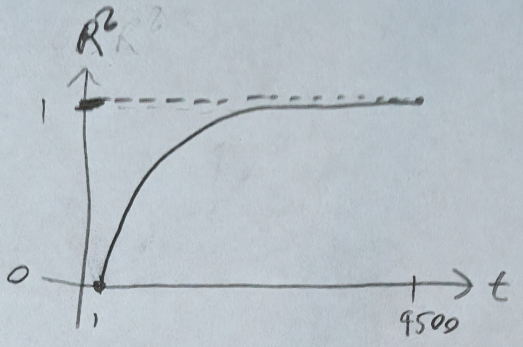
\includegraphics[width=0.4\linewidth]{in_sample_Rsq.png}
\end{figure}
}}{~\spc{3.5}}

\subquestionwithpoints{4} Draw the oos$R^2$ by the iteration number. Label your axes (y is oos$R^2$ and x is $t$). Label critical points on both the x and y axes.

\iftoggle{solutions}{\inred{
\begin{figure}[h]
    \centering
    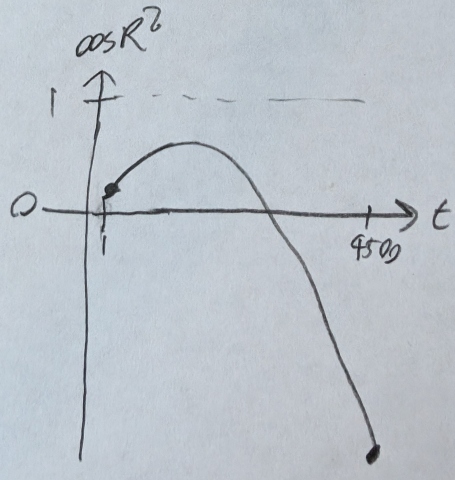
\includegraphics[width=0.3\linewidth]{oos_Rsq.png}
\end{figure}

Note: the oos$R^2$ point at $t=1$ will be positive or negative but approximately zero but its true value is unknown and the oos$R^2$ point at $t=4500$ will be negative but its true value is unknown.
}}{~\spc{4}}
\pagebreak

We now model arrival delay using a regression tree with the default hyperparameter value of $N_0  = 5$ for regression:

\begin{Verbatim}
> tree_mod = YARFCART(X_train, y_train)
\end{Verbatim}

and print out an illustration of \texttt{tree\_mod} to depth 3:
 
\begin{figure}[h]
    \centering
    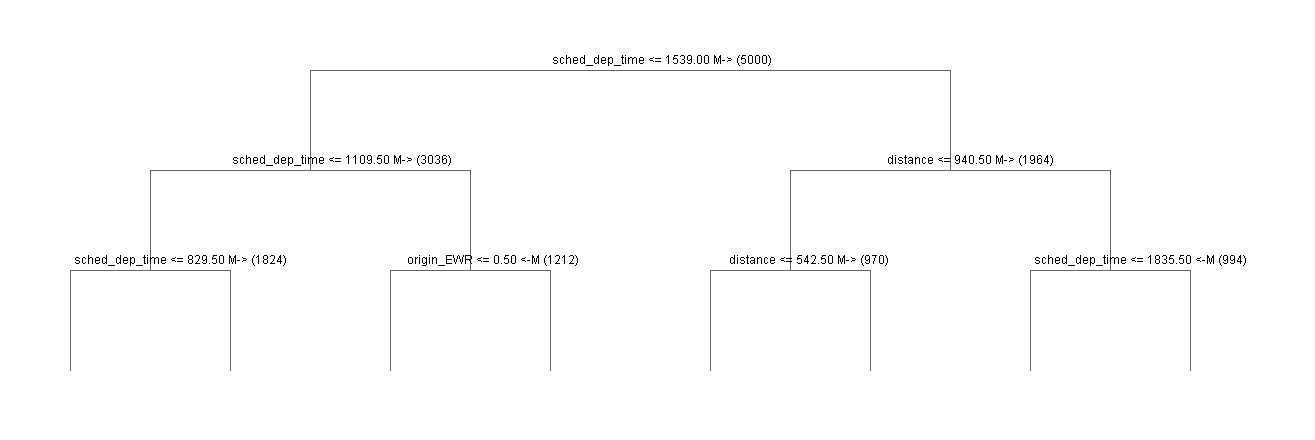
\includegraphics[width=1.1\linewidth]{yarf_mod_tree_1.png}
\end{figure}


\subquestionwithpoints{1} Assuming the tree model above, what is the most important variable?

\iftoggle{solutions}{\inred{
\texttt{sched\_dep\_time}
}}{~\spc{-0.25}}

\subquestionwithpoints{1} Assuming the tree model above, what is the second most important variable?

\iftoggle{solutions}{\inred{
\texttt{distance}
}}{~\spc{-0.25}}

Also compute a linear model:

\begin{Verbatim}
> ols_mod = lm(y_train ~ ., X_train)
\end{Verbatim}

\subquestionwithpoints{1} Assume the real function $f$ has many non-linearities and interactions among the $p_{raw}$ features. Which model would likely perform better in the future? \\ Circle one...  ~~\texttt{ols\_mod}~~/~~\iftoggle{solutions}{\inred{\texttt{tree\_mod}}}{\texttt{tree\_mod}}

\subquestionwithpoints{1} Assume the real function $f$ does not have many non-linearities and interactions among the $p_{raw}$ features. Which model would likely perform better in the future? \\ Circle one...  ~~\iftoggle{solutions}{\inred{\texttt{ols\_mod}}}{\texttt{ols\_mod}} ~~/~~\texttt{tree\_mod}


\subquestionwithpoints{3} Assuming you cannot use different training data, how can you improve the oos performance during fitting a single regression tree?

\iftoggle{solutions}{\inred{
Use the model selection procedure to optimize the hyperparameter value $N_0$.
}}{~\spc{0.5}}
\end{enumerate}


\pagebreak

\noindent We now model arrival delay using a bag-of-trees model and a Random Forests model where in the latter we use the default hyperparameter value of floor($p_{raw}/3$):

\begin{Verbatim}
> bag_tree_mod = YARFBAG(X_train, y_train, num_trees = 2000)
> bag_tree_mod$rmse_oob
[1] 43.3813
> rf_mod = YARF(X_train, y_train, num_trees = 2000)
> rf_mod$rmse_oob
[1] 42.6371
\end{Verbatim}
\begin{enumerate}[(aa)]





\subquestionwithpoints{1} Which model is more interpretable? \\ Circle one...  ~~\texttt{rf\_mod} ~~/~~\texttt{bag\_tree\_mod}~~/~~\iftoggle{solutions}{\inred{\texttt{tree\_mod}}}{\texttt{tree\_mod}}


\subquestionwithpoints{1} Which model would likely perform better in the future? \\ Circle one...  ~~\iftoggle{solutions}{\inred{\texttt{rf\_mod}}}{\texttt{rf\_mod}} ~~/~~\texttt{bag\_tree\_mod}~~/~~\texttt{tree\_mod}


\subquestionwithpoints{2} If \texttt{rf\_mod} was instead fit with $m_{try} = 1$, which model would likely perform better in the future?  \\ Circle one...  ~~\texttt{rf\_mod} ~~/~~\iftoggle{solutions}{\inred{\texttt{bag\_tree\_mod}}}{\texttt{bag\_tree\_mod}}~~/~~\texttt{tree\_mod}



\subquestionwithpoints{2} Assuming you cannot use different training data, and assuming 2,000 trees is sufficient, how can you improve the oos performance during fitting the random forest model?

\iftoggle{solutions}{\inred{
Use the model selection procedure to optimize the hyperparameter value $m_{try}$.
}}{~\spc{1}}

\subquestionwithpoints{6} Fill in the blanks in following terms using one of the following symbols $>,<,\geq,\leq,=,?$ where \qu{?} should be used only if the comparison is not possible. Express the relationships that are expected (those that we spent time studying in class).\\

Bias of \texttt{tree\_mod}  \iftoggle{solutions}{\inred{$=$}}{~\line(1,0){15}~} Bias of \texttt{bag\_tree\_mod}      \iftoggle{solutions}{\inred{$=$}}{~\line(1,0){15}~}     Bias of \texttt{rf\_mod}   \iftoggle{solutions}{\inred{$<$}}{~\line(1,0){15}~}      Bias of \texttt{ols\_mod} \\

Var of \texttt{tree\_mod}  \iftoggle{solutions}{\inred{$>$}}{~\line(1,0){15}~}      Var of \texttt{bag\_tree\_mod}      \iftoggle{solutions}{\inred{$>$}}{~\line(1,0){15}~}      Var of \texttt{rf\_mod}   \iftoggle{solutions}{\inred{$>$}}{~\line(1,0){15}~}     Var of \texttt{ols\_mod} \\

MSE of \texttt{tree\_mod}  \iftoggle{solutions}{\inred{$>$}}{~\line(1,0){15}~}      MSE of \texttt{bag\_tree\_mod}      \iftoggle{solutions}{\inred{$>$}}{~\line(1,0){15}~}      MSE of \texttt{rf\_mod}   \iftoggle{solutions}{\inred{$<$}}{~\line(1,0){15}~}     MSE of \texttt{ols\_mod}

\pagebreak


We now model arrival delay using the boosting model we discussed in class with 2,000 shallow trees as the base learner:


\begin{Verbatim}
> Xmm = model.matrix(~ ., X)
> boost_mod = xgboost(
    data = Xmm[idx_train, ], 
    label = y_train,
    objective = "reg:squarederror", #for a regression problem
    booster = "gbtree", #shallow trees, default depth = 6
    nrounds = 2000, #num trees (should be cross-validated)
    eta = 0.2, #learning rate (should be cross-validated)
    print_every_n = 100
  )

> n_test = 500
> y_hat_test = predict(boost_mod, Xmm[idx_test, ][1 : n_test, ])
> sqrt(mean((y_test[1 : n_test] - y_hat_test)^2)) #oosRMSE calculation
[1] 39.06686
\end{Verbatim}


\subquestionwithpoints{1} Which model would likely perform better in the future? \\ Circle one...  ~~\texttt{rf\_mod}~~/~~\iftoggle{solutions}{\inred{\texttt{boost\_mod}}}{\texttt{boost\_mod}}

\subquestionwithpoints{1} Which model likely has less estimation error? \\ Circle one...  ~~\texttt{rf\_mod}~~/~~\iftoggle{solutions}{\inred{\texttt{boost\_mod}}}{\texttt{boost\_mod}}

\subquestionwithpoints{2} Which model likely has less stability in its estimate of future RMSE? \\ Circle one...  ~~\texttt{rf\_mod}~~/~~\iftoggle{solutions}{\inred{\texttt{boost\_mod}}}{\texttt{boost\_mod}}

\subquestionwithpoints{2} Which model has more hyperparameter values to optimize? \\ Circle one...  ~~\texttt{rf\_mod}~~/~~\iftoggle{solutions}{\inred{\texttt{boost\_mod}}}{\texttt{boost\_mod}}

\subquestionwithpoints{3} Fill in the blanks in following terms using one of the following symbols $>,<,\geq,\leq,=,?$ where \qu{?} should be used only if the comparison is not possible. Express the relationships that are expected (those that we spent time studying in class).\\

Bias of \texttt{rf\_mod}   \iftoggle{solutions}{\inred{$?$}}{~\line(1,0){15}~}      Bias of \texttt{boost\_mod} \\

Var of \texttt{rf\_mod}   \iftoggle{solutions}{\inred{$?$}}{~\line(1,0){15}~}     Var of \texttt{boost\_mod} \\

MSE of \texttt{rf\_mod}   \iftoggle{solutions}{\inred{$?$}}{~\line(1,0){15}~}     MSE of \texttt{boost\_mod}

\pagebreak


We are now interested in changing the response to the following binary response: 1 if the flight is delayed by more than a half hour (i.e. if the previous metric $y > 30$) or if the flight is not (i.e. if the previous metric $y \leq 30$). We fit a logistic regression to the raw features. 

\begin{Verbatim}[fontsize=\small]
> y_train_bin = as.numeric(y_train > 30)
> table(y_train_bin)
y_train_bin
   0    1 
4205  795
> logistic_mod = glm(y_train_bin ~ . - model, X_train, family = "binomial")
\end{Verbatim}

Below is a subset of the coefficients in the fit $\b$:

\begin{Verbatim}[fontsize=\small]
> coef(logistic_mod)
   (Intercept) sched_dep_time sched_arr_time 
 -1.975068e+01   1.317949e-03   3.681219e-05 
     carrierAA      carrierAS      carrierB6 
 -3.699871e-01  -1.802762e-01   3.718844e-02 
     carrierDL      carrierEV      carrierF9 
 -5.471695e-01   3.698079e-01   7.164400e-01 
     carrierFL      carrierHA      carrierMQ 
  1.374622e-01  -1.399129e+01  -2.033716e-01 
     carrierUA      carrierUS      carrierVX 
 -2.642582e-01  -3.790116e-01   8.489270e-02 
     carrierWN      carrierYV      originJFK 
  2.818394e-01   3.628071e-01  -3.211934e-01  
     originLGA        destACK        destALB 
 -4.340381e-01   4.986711e+01   4.930801e+01 
\end{Verbatim}


\subquestionwithpoints{1} circle one: Assuming you use the model \texttt{logistic\_mod}, relative to Newark airport (the reference level of variable \texttt{origin}), you are ... \\

~~more~~ / ~~\iftoggle{solutions}{\inred{less}}{less}~~ \\ 

likely to be delayed by 30min or more if the origin is JFK.

\subquestionwithpoints{3} Using the model \texttt{logistic\_mod}, you predict for your flight tomorrow (with measurements $\x_{\star}$) and compute $\x_{\star} \b = 3.171$. What is the predicted probability of a more than 30 min arrival delay to the nearest three decimals?

\iftoggle{solutions}{\inred{
\beqn
\frac{e^{3.171}}{1 + e^{3.171}} = 0.960 = 95.973\%
\eeqn
}}{~\spc{3}}

\pagebreak



\subquestionwithpoints{2} Our \texttt{logistic\_mod}'s oos Brier score is $-0.121$. Does \texttt{logistic\_mod} beat the naive probability estimation model where you let $\hat{p} = 0.5$ for all predicted units? Explain.

\iftoggle{solutions}{\inred{
Yes. It has a higher Brier score than the naive model whose Brier score is -0.25.\\
}}{~\spc{1.5}}

We now compute the oos ROC curve for \texttt{logistic\_mod} and illustrate it below.

\begin{figure}[h]
    \centering
    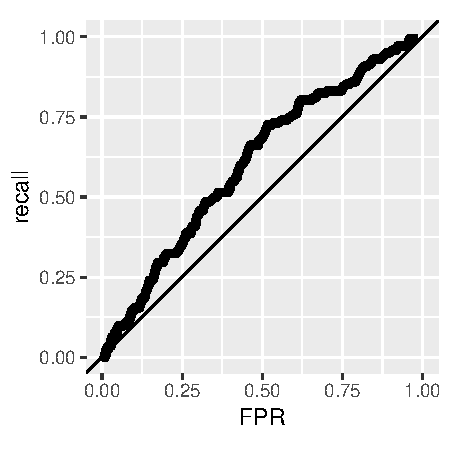
\includegraphics[width=0.5\linewidth]{roc}
\end{figure}

\subquestionwithpoints{1} Estimate the oos AUC.

\iftoggle{solutions}{\inred{
Since the upper triangle has area 0.5, I estimate the curve has about 15\% of the area, so I'm estimating 0.55-0.65.
}}{~\spc{1.5}}

\subquestionwithpoints{1} Circle one: the in-sample AUC is likely...  \\

~~lower than~~ / ~~\iftoggle{solutions}{\inred{higher than}}{higher than}~~~~ the oos AUC.



\subquestionwithpoints{2} Circle one: the easiest way to improve the AUC is likely to...  \\

increase the training set size and fit the same model~~ / \\ ~~\iftoggle{solutions}{\inred{add interactions and quadratic terms and fit a different model}}{add interactions and quadratic terms and fit a different model}~~ \\ 

\pagebreak

\begin{Verbatim}[fontsize=\small]
> table(y_test_bin, as.numeric(p_hat_test > 0.025))
          
y_test_bin   0   1
         0  19 839
         1   1 141
         
> table(y_test_bin, as.numeric(p_hat_test > 0.05))
          
y_test_bin   0   1
         0  96 762
         1   7 135
> table(y_test_bin, as.numeric(p_hat_test > 0.1))
          
y_test_bin   0   1
         0 419 439
         1  41 101
> table(y_test_bin, as.numeric(p_hat_test > 0.2))
          
y_test_bin   0   1
         0 692 166
         1  98  44
> table(y_test_bin, as.numeric(p_hat_test > 0.3))
          
y_test_bin   0   1
         0 804  54
         1 128  14
> table(y_test_bin, as.numeric(p_hat_test > 0.4))
          
y_test_bin   0   1
         0 846  12
         1 139   3
\end{Verbatim}

\subquestionwithpoints{2}  We are interested in minimizing the error that occurs in the future when we (1) predict the flight is not delayed by more than 30min and then (2) in reality it is delayed by more than 30min. Of the asymmetric models shown above, which value of $p_{th}$ would optimize for our goal?

\iftoggle{solutions}{\inred{
0.025
}}{~\spc{1}}

\subquestionwithpoints{3} Assuming you chose the model in the previous question, what is the tradeoff if you use this model in the future?

\iftoggle{solutions}{\inred{
You make many false positive errors.
}}{~\spc{1}}




\end{enumerate}

\end{document}


\problem This question relates to conceptual issues.


\begin{enumerate}[(a)]

\subquestionwithpoints{8} Circle the letters of all the following that are \textbf{true}. The notation below should be assumed the same from class. \iftoggle{solutions}{\inred{
c d f i j k m n
}}

\begin{enumerate}[(a)]
\item A model $g$ for a real-world, non-man-made phenomenon $y$ which is a function of real-world measurements $x-1, \ldots, x-p$ could be absolutely true, (i.e. always have zero error when predicting in for future units).
\item A model $g$ for phenomenon $y$ can be proved true analytically (using a mathematical deductive proof).
\item A null model $g-0$ outputs a value in the set $\mathcal{Y}$.
\item A null model $g-0$ can still be \qu{useful} to the model's user.
\item Any model $g$ which is a function of real-world measurements $x-1, \ldots, x-p$ \textit{always} beats $g-0$ on predictive performance.
\item A model $g$ for phenomenon $y$ which is of type nominal categorical with possible values within the set $C-1, C-2, \ldots, C-L$ must return a value within the set $C-1, C-2, \ldots, C-L$.
\item A model $g$ for phenomenon $y$ which is of type nominal categorical with possible values within the set $C-1, C-2, \ldots, C-L$ must have a proxy $x-j$ which is also type nominal categorical with possible values within the set $C-1, C-2, \ldots, C-L$.

\item If $x-j$ is of type nominal categorical with possible values within the set $C-1, C-2, \ldots, C-L$, then it is reasonable when modeling that those categorical values should be replaced by $1, 2, \ldots, L$.

\item If $x-j$ is of type nominal categorical with possible values within the set $C-1, C-2, \ldots, C-L$, then it is reasonable when modeling that those categorical values should be replaced by $L-1$ binary variables indicating the presence of absence of categories $C-2, \ldots, C-L$.

\item If $x-j$ is of type ordinal with possible values within the set $C-1, C-2, \ldots, C-L$, assuming that set is ordered from smallest to largest, then it is reasonable when modeling that those categorical values \textit{can} be replaced by $1, 2, \ldots, L$.

\item If $x-j$ is of type ordinal with possible values within the set $C-1, C-2, \ldots, C-L$, then it is reasonable when modeling that those categorical values \textit{can} be replaced by $L-1$ binary variables indicating the presence of absence of categories $C-2, \ldots, C-L$.

\item In-sample performance metrics gives you an honest idea about how accurate your model is when using it for future prediction \textit{always}.
\item In-sample performance metrics gives you an honest idea about how accurate your model is when using it for future prediction \textit{only} when $n$ is much larger than $p$.
\item Out-of-sample validation gives you an idea about how accurate your model is when using it for future prediction \textit{always}.
\item Out-of-sample validation gives you an idea about how accurate your model is when using it for future prediction \textit{only} when $n$ is much larger than $p$.
\item Out-of-sample validation gives you an idea about how accurate your model is when using it for future prediction \textit{only} when $\mathcal{Y} \subseteq \reals$.
\end{enumerate}

\end{enumerate}
\pagebreak

\problem Consider the following data frame $\mathbb{D}$. Below is some \texttt{R} code (lines beginning with $>$ are commands that were entered, other lines are output from those commands).

\begin{lstlisting}
> skimr::skim(D)
--- Data Summary ---------------------------------  
                           Values
Name                       D     
Number of rows             592   
Number of columns          4     
Key                        NULL  
---------------------------------           
Column type frequency:           
  character                2     
  numeric                  2     
---------------------------------         
Group variables            None  

--- Variable type: factor ---------------------
  skim_variable n_missing complete_rate ordered n_unique top_counts                           
1 eye-color             0             1 FALSE          4 Bro: 220, Blu: 215, Haz: 93, Gre: 64 
2 hair-color            0             1 FALSE          4 Bro: 286, Blo: 127, Bla: 108, Red: 71

--- Variable type: numeric ------------------
  skim_variable n_missing complete_rate  mean    sd p0 p25 p50 p75 p100 
1 is-male               0             1 0.471 0.500  0   0   0   1    1 
2 is-not-male           0             1 0.529 0.500  0   0   1   1    1 

> D$is-not-male = 1 - D$is-male
> D[sample(1 : nrow(D), 10), ]
    is-male eye-color hair-color is-not-male
71        1     Brown      Brown           0
446       0     Hazel      Brown           1
474       0     Green      Brown           1
75        1     Brown      Brown           0
489       0     Brown        Red           1
107       1     Brown      Brown           0
473       0     Green      Brown           1
69        1     Brown      Brown           0
447       0     Hazel      Brown           1
137       1      Blue      Brown           0
\end{lstlisting}

\begin{enumerate}[(a)]

\subquestionwithpoints{1} Circle one letter: the output on lines 28--37 is ... 

\begin{enumerate}[A)]
    \item the first 10 rows of data frame $\mathbb{D}$
    \item \iftoggle{solutions}{\inred{
a random 10 rows of data frame $\mathbb{D}$
}}{
a random 10 rows of data frame $\mathbb{D}$
}
    \item the last 10 rows of data frame $\mathbb{D}$
\end{enumerate}
\pagebreak

\subquestionwithpoints{1} What type of variable is \texttt{eye\-color}? Be as specific as you can.

\iftoggle{solutions}{\inred{
nominal (or unordered) categorical (or factor)
}}{~\spc{1}}

Let $y$ be defined as the variable \texttt{is\-male} and all other variables be considered features.


\subquestionwithpoints{2} What is the $g-0$ function equal to explicitly?

\iftoggle{solutions}{\inred{
$g-0 = $ 0
}}{~\spc{0.5}}

\subquestionwithpoints{3}  Circle all of the following modeling procedures that would be appropriate for this modeling setting considering the response space.

\begin{enumerate}[A)]
    \item OLS
    \item \iftoggle{solutions}{\inred{
Perceptron
}}{
Perceptron
}
    \item \iftoggle{solutions}{\inred{
SVM
}}{
SVM
}
    \item \iftoggle{solutions}{\inred{
SVM with Vapnik objective function (and a numeric choice for hyperparameter $\lambda$)
}}{
SVM with Vapnik objective function (and a numeric choice for hyperparameter $\lambda$)
}
    \item \iftoggle{solutions}{\inred{
KNN with the Euclidean distance function
}}{
KNN with the Euclidean distance function
}
    \item \iftoggle{solutions}{\inred{
KNN with a non-Euclidean, but still valid distance function
}}{
KNN with a non-Euclidean, but still valid distance function
}
\end{enumerate}


\subquestionwithpoints{3} Regardless of your answer in (c), how many columns will the full-rank design matrix $X$ have? Hint: make sure you include the $\onevec-n$ as the first column in $X$.

\iftoggle{solutions}{\inred{
8 = 1 for intercept + 3 for eye\-color + 3 for hair\-color + 1 for is\-not\-male
}}{~\spc{0.5}}


\subquestionwithpoints{2} Regardless of your answer in (c), consider using the SVM to fit $g$. What would the in-sample misclassification error for $g$ be?

\iftoggle{solutions}{\inred{
0
}}{~\spc{1}}


\subquestionwithpoints{2} Regardless of your answer in (c), consider using the OLS to fit $g$. What would the in-sample misclassification error for $R^2$ be?

\iftoggle{solutions}{\inred{
1
}}{~\spc{1}}

\pagebreak
Now we will change the modeling target. Let $y$ be defined as the variable \texttt{eye\-color} and all other variables be considered features.


\subquestionwithpoints{2} What is the $g-0$ function equal to explicitly?

\iftoggle{solutions}{\inred{
$g-0 = $ Brown
}}{~\spc{0}}

\subquestionwithpoints{3}  Circle all of the following modeling procedures that would be appropriate for this modeling setting considering the response space.

\begin{enumerate}[A)]
    \item OLS
    \item Perceptron
    \item SVM
    \item SVM with Vapnik objective function (and a numeric choice for hyperparameter $\lambda$)

    \item \iftoggle{solutions}{\inred{
KNN with the Euclidean distance function
}}{
KNN with the Euclidean distance function
}
    \item \iftoggle{solutions}{\inred{
KNN with a non-Euclidean, but still valid distance function
}}{
KNN with a non-Euclidean, but still valid distance function
}
\end{enumerate}


\subquestionwithpoints{3} Regardless of your answer in (g), how many columns will the full-rank design matrix $X$ have? Hint: make sure you include the $\onevec-n$ as the first column in $X$.

\iftoggle{solutions}{\inred{
5 = 1 for intercept + 3 for hair\-color + 1 for is\-male (this is\-not\-male is dropped as it's a linear combination of the intercept and is\-male)
}}{~\spc{0.5}}

Now we will change the modeling target again. Let $y$ be defined as the variable \texttt{hair\-color} and we only use the feature \texttt{eye\-color}.

\subquestionwithpoints{5} Let the reference level of \texttt{eye\-color} be Green. For the subset of the data shown on rows 28--37 of the code, provide the same 10-row subset of the full-rank design matrix $X$. Name the columns of $X$ appropriately.


\iftoggle{solutions}{
\begin{table}[h]
    \centering
    \inred{
    \begin{tabular}{|c|c|c|c|}
        (intercept) & eye\-color\-is\-brown & eye\-color\-is\-blue & eye\-color\-is\-hazel  \\ \hline
        1 & 1 & 0 & 0 \\
        1 & 0 & 0 & 1 \\
        1 & 0 & 0 & 0 \\
        1 & 1 & 0 & 0 \\
        1 & 1 & 0 & 0 \\
        1 & 1 & 0 & 0 \\
        1 & 0 & 0 & 0 \\
        1 & 1 & 0 & 0 \\
        1 & 0 & 0 & 1 \\
        1 & 0 & 1 & 0 \\ \hline
    \end{tabular}}
\end{table}
}{~\spc{6}}
\pagebreak

\subquestionwithpoints{2} Assume you use KNN with the Euclidean distance function to fit $g$. Of the three sources of error, which is likely the largest source of error in $g$'s predictions?

\iftoggle{solutions}{\inred{
ignorance
}}{~\spc{0.5}}
\end{enumerate}


\problem Here are some theoretical questions. For all notation used, assume it has the same as it did in class.


\begin{enumerate}[(a)]

\subquestionwithpoints{4} Assume $\mathcal{A} = $ OLS (linear regression). Prove that $\bv{b} = R^{-1} Q^\top \y$.


\iftoggle{solutions}{\inred{
\beqn
\b &=& (X^\top X)^{-1} X^\top \y \\
&=& ((QR)^\top QR)^{-1} (QR)^\top \y \\
&=& (R^\top Q^\top QR)^{-1} R^\top Q^\top \y \\
&=& (R^\top R)^{-1} R^\top Q^\top \y \\
&=& R^{-1} (R^\top)^{-1} R^\top Q^\top \y \\
&=& R^{-1} Q^\top \y \\
\eeqn
}}{~\spc{6}}

\subquestionwithpoints{10} Assume $\mathcal{A} = $ OLS (linear regression). For each of the following, if the operation is illegal, write \qu{illegal}. If the operation is legal and the expression allows for simplification, simplify as best you can after an \qu{=} sign. If you cannot simplify, then leave the line \textit{blank}. If your answer is the zero or one vector, please indicate the dimension as a subscript to get full credit.

\begin{itemize}
    \item $XQ$ \iftoggle{solutions}{\inred{
illegal
}}{~\spc{0.5}}
    \item $XR$ \iftoggle{solutions}{\inred{

}}{~\spc{0.5}}
    \item $X\bv{b}$ \iftoggle{solutions}{\inred{
$= \hat{\y}$
}}{~\spc{0.5}}
    \item $HQ$ \iftoggle{solutions}{\inred{
$= Q$
}}{~\spc{0.5}}
\pagebreak
    \item $QH$ \iftoggle{solutions}{\inred{
illegal
}}{~\spc{0.5}}
    \item $Q\bv{b}$ \iftoggle{solutions}{\inred{

}}{~\spc{0.5}}
    \item $\y^\top H$ \iftoggle{solutions}{\inred{
$= \hat{\y}^\top$
}}{~\spc{0.5}}
    \item $\bv{e}^\top H$ \iftoggle{solutions}{\inred{
$= \zerovec-n^\top$
}}{~\spc{0.5}}
    \item $QQ^\top \onevec-n$ \iftoggle{solutions}{\inred{
$= \onevec-n$
}}{~\spc{0.5}}
    \item $\rank{H} / \rank{X}$ \iftoggle{solutions}{\inred{
$= 1$
}}{~\spc{0}}
\end{itemize}



\end{enumerate}

\problem Consider the Galton dataset we examined in lab. Below is some \texttt{R} code (lines beginning with $>$ are commands that were entered, other lines are output from those commands).

\begin{lstlisting}
> skimr::skim(HistData::Galton)
--- Data Summary ------------------------
                           Values          
Name                       HistData::Galton
Number of rows             928             
Number of columns          2               
-------------------------                  
Column type frequency:                     
  numeric                  2                

--- Variable type: numeric ------------------------- 
  skim_variable n_missing complete_rate mean   sd   p0  p25  p50  p75 p100 
1 parent                0             1 68.3 1.79 64   67.5 68.5 69.5 73   
2 child                 0             1 68.1 2.52 61.7 66.2 68.2 70.2 73.7 
\end{lstlisting}

\vspace{-0.7cm}

\begin{enumerate}[(a)]

\subquestionwithpoints{1} What is the sample size of this dataset?

\iftoggle{solutions}{\inred{
$928$
}}{~\spc{0}}
\pagebreak


As in the lab, consider the dependent variable \texttt{child} which measures the height of a child and consider the independent variable \texttt{parent} which measures the average height of the mother and father of the child.

\subquestionwithpoints{1} What is $p$ in this modeling context?

\iftoggle{solutions}{\inred{
$1$
}}{~\spc{0}}

\subquestionwithpoints{3} \qu{The unit is one \-\-\-} (fill in the blank below by describing the unit).

\iftoggle{solutions}{\inred{
father-mother-child trio
}}{~\spc{2}}


\subquestionwithpoints{2} Regardless of the $\mathcal{A}$ employed to create a model, which will likely be the greatest of the three sources of error?

\iftoggle{solutions}{\inred{
ignorance (since there's only one feature and the phenomenon of interest is complicated)
}}{~\spc{1}}

\subquestionwithpoints{2} If $\mathcal{A} =$ OLS, what are the contents of the set $\mathcal{H}$?

\iftoggle{solutions}{\inred{
\beqn
\mathcal{H} = \braces{w-0 + w-1 x : w-0, w-1 \in \reals} = \braces{[1~x]\bv{w} : \bv{w} \in \reals^2}
\eeqn
}}{
$~\\\mathcal{H} = $~\spc{1}}

\subquestionwithpoints{3} If $\mathcal{A} =$ OLS, provide one specific $<x,y>$ point on the OLS line (i.e. the $g$ model).

\iftoggle{solutions}{\inred{
since $<\xbar, \ybar>$ is always on the OLS line, the only point you could know about without more output is $<68.3, 68.1>$ 
}}{~\spc{1.5}}

\pagebreak

\subquestionwithpoints{5} Prove numerically that there is \qu{regression to the mean} for the phenomenon of interest in this modeling setting. Assume that the correlation coefficient between the two variables is 0.46.

\iftoggle{solutions}{\inred{
Regression to the mean means that we predict a child to have a smaller height than their parents for parents with above-average height and we predict a child to have a larger height than their parents for parents with below-average height. This is equivalent to showing $b-1 < 1$. We now calculate $b-1$ and show it is less than 1.

\beqn
b-1 = r \frac{s-y}{s-x} = 0.46 \cdot \frac{2.52}{1.79} = 0.65 < 1
\eeqn
}}{~\spc{5}}


\subquestionwithpoints{5} If $\mathcal{A} =$ OLS, calculate the RMSE to two decimals.

\iftoggle{solutions}{\inred{
\beqn
SST &=& (n-1)s^2-y = 927 \cdot 2.52^2 = 5886.821 \\
R^2 &=& 1 - SSE / SST \mathimplies SSE = SST (1 - R^2) = 5886.821 (1 - .46^2) = 4650.588 \\
RMSE &=& \sqrt{\frac{SSE}{n - (p+1)}} = \sqrt{\frac{4650.588}{ 926}} = 2.24
\eeqn
}}{~\spc{5.5}}

\end{enumerate}

\problem Consider the following illustration of cross-validation for $\mathbb{D}$ with $n=200$.

\begin{figure}[h]
    \centering
    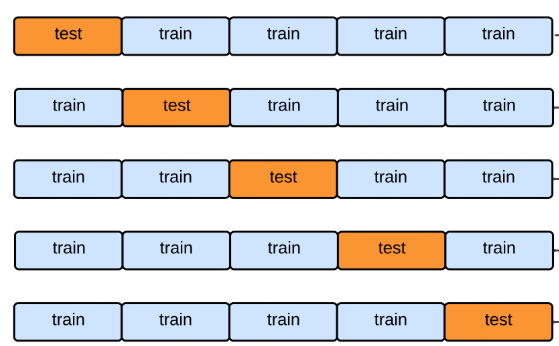
\includegraphics[width=3.5in]{cv.png}
\end{figure}
\FloatBarrier
\pagebreak

\begin{enumerate}[(a)]

\subquestionwithpoints{1} What is the value of $K$?

\iftoggle{solutions}{\inred{
5
}}{~\spc{0}}

\subquestionwithpoints{1} How many units will be in $\mathbb{D}-{train}$ in the first split?

\iftoggle{solutions}{\inred{
$n - \oneover{K} n = 160$
}}{~\spc{0}}

\subquestionwithpoints{1} If you calculate oos residuals in the second split, how many oos residuals will there be?

\iftoggle{solutions}{\inred{
It's the same as the size of $\mathbb{D}-{test}$ which is 40.
}}{~\spc{0}}


\subquestionwithpoints{2} If $g$ was overfit on $\mathbb{D}-{train}$, then how would oosRMSE be expected to compare with in-sample RMSE?

\iftoggle{solutions}{\inred{
oosRMSE $>$ in-sample RMSE
}}{~\spc{3}}

\subquestionwithpoints{3} If you calculate the oosRMSE from the residuals in (c), this oosRMSE is expected to be greater than, less than or equal to the oosRMSE you expect in the future when predicting on $g-{final}$ which is fit with all $\mathbb{D}$?

\iftoggle{solutions}{\inred{
greater than
}}{~\spc{3}}

\subquestionwithpoints{3} If you aggregate all the residuals from all $K$ folds together and calculate the oosRMSE, this oosRMSE is expected to be greater than, less than or equal to the oosRMSE you expect in the future when predicting on $g-{final}$ which is fit with all $\mathbb{D}$?

\iftoggle{solutions}{\inred{
greater than
}}{~\spc{3}}

\end{enumerate}
\pagebreak

\problem Consider the following $\mathbb{D}$ illustrated within the questions below.



\begin{enumerate}[(a)]

\subquestionwithpoints{2} Examine the plot of $\mathbb{D}$ in the following question. If $y$ is the response variable and the other two variables are considered features, what is the formal name of the type of modeling scenario most likely depicted?

\iftoggle{solutions}{\inred{
binary classification
}}{~\spc{1}}

\subquestionwithpoints{2} If $\mathcal{A} = $ perceptron with the $\mathcal{H}$ we considered thus far in class, draw a possible $g$ that outputs from this algorithm after 10,000 iterations on the illustration below:

\begin{figure}[h]
    \centering
    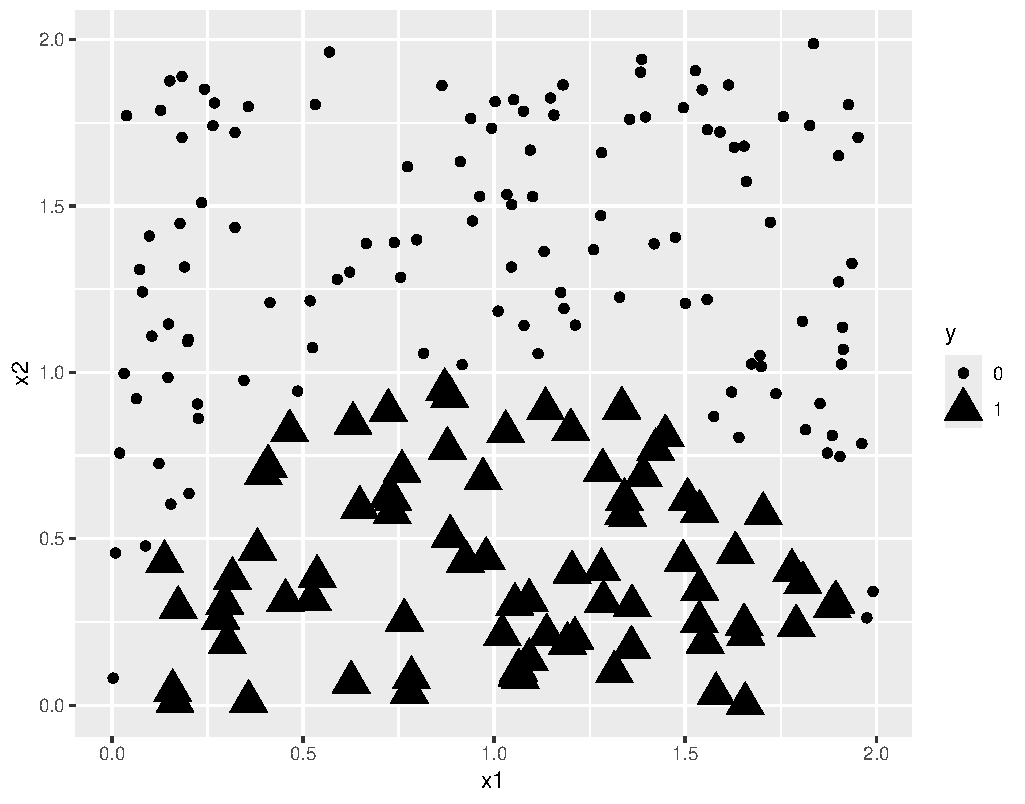
\includegraphics[width=5in]{classification.pdf}
\end{figure}
\FloatBarrier

\iftoggle{solutions}{\inred{
any straight line is acceptable
}}{~\spc{-1}}


\subquestionwithpoints{1} If $\mathcal{A} = $ perceptron with the $\mathcal{H}$ we considered thus far in class, will the algorithm eventually converge? Circle one: ~~yes~~/~~\iftoggle{solutions}{\inred{no}}{no}

\pagebreak

\subquestionwithpoints{4} If $\mathcal{A} = $ SVM with the $\mathcal{H}$ we considered thus far in class and the Vapnik function with hinge errors and $\lambda = 0.001$, draw the $g$ that most likely outputs from this algorithm on the illustration below:

\begin{figure}[h]
    \centering
    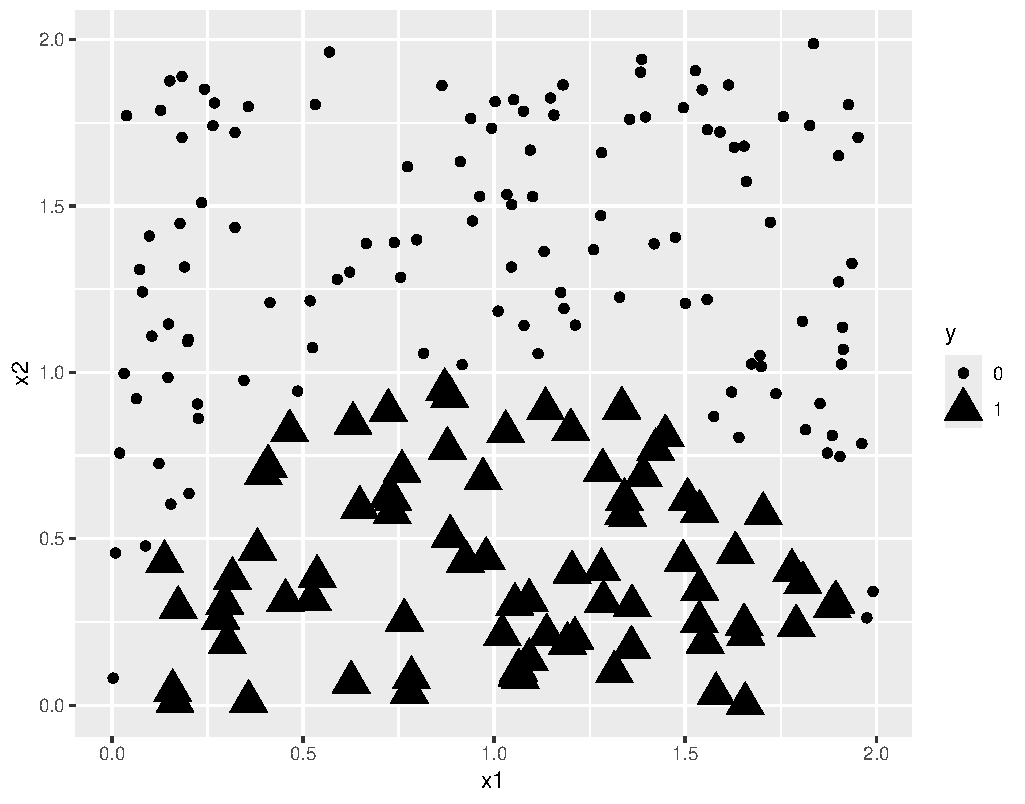
\includegraphics[width=5in]{classification.pdf}
\end{figure}
\FloatBarrier

\iftoggle{solutions}{\inred{
With the hyperparameter set to such a low value, we're really just minimizing sum of hinge errors which would likely be the horizontal line at $x-2 \approx 0.75$.
}}{~\spc{-1}}


\subquestionwithpoints{3} If $\mathcal{A} = $ SVM with the $\mathcal{H}$ we considered thus far in class and the Vapnik function with hinge errors and $\lambda = 0.001$, what is the most likely of the three sources of error in $g$?

\iftoggle{solutions}{\inred{
Misspecification since we can clearly see a semicircle threshold with diameter running across $x-2 = 0$ can obtain near zero misclassification error.
}}{~\spc{1}}



\subquestionwithpoints{2} If $\mathcal{A} = $ KNN with the Euclidean distance function and $K=1$, what would be $g(0,0)$?

\iftoggle{solutions}{\inred{
The closest point to $<0,0>$ has $y = 0$ so thus $\yhat = 0$.
}}{~\spc{1}}

\subquestionwithpoints{2} If $\mathcal{A} = $ KNN with the Euclidean distance function and $K=10$, what would be $g(0,0)$?

\iftoggle{solutions}{\inred{
Draw a circle arc from the y-axis to the x-axis with $<0,0>$ at its center such that 10 points are included. It is clear that there are more triangles than dots so that the modal value $\yhat = 1$.
}}{~\spc{1}}

\end{enumerate}

\end{document}

\problem We measure the time (in months) between $n=60$ earthquakes. Here is a scatterplot of the raw data:

\begin{figure}[h]
    \centering
    \includegraphics[width=4.5in]{earthquake-plot.pdf}
    \label{fig:enter-label}
\end{figure}

The time between earthquakes is known to be exponentially distributed. We suspect the distribution's mean changed once (at some point). So the DGP for the above data will be:

\beqn
X-1, X-2, \ldots, X-{\theta-3} \iid \theta-1 e^{-\theta-1 x} ~~\text{independent of}~~ X-{\theta-3 + 1}, X-{\theta-3 + 2}, \ldots, X-n \iid \theta-2 e^{-\theta-2 x}
\eeqn

\noindent For this problem, you may need to know some of these facts about the gamma distribution:

\beqn
Y \sim \text{Gamma}(\alpha, \beta) := \frac{\beta^\alpha}{\Gamma(\alpha)} y^{\alpha - 1} e^{-\beta y} \indic{y > 0}, ~~ F(y) = P(\alpha, \beta y),~~S(y) = Q(\alpha, \beta y)
\eeqn

\noindent where $P,Q$ are the lower and upper regularized gamma functions.

\begin{enumerate}[(a)]

\subquestionwithpoints{2} How many parameters can you draw inference for in this DGP?
%
\iftoggle{solutions}{\inred{
\beqn
3
\eeqn
}}{~\spc{0.5}}
%

\subquestionwithpoints{5} Find the likelihood of the data, $f(\x; \theta-1, \theta-2, \theta-3)$. Denote the sample size as $n$ i.e., do not use its known value of 60 here. You can assume all $x-i > 0$.
%
\iftoggle{solutions}{\inred{
\beqn
f(\x; \theta-1, \theta-2, \theta-3) &=& \prod-{i=1}^{\theta-3} f(x-i; \theta-1) \prod-{\theta-3 +1}^n f(x-i; \theta-2) \\
 &=& \prod-{i=1}^{\theta-3} \theta-1 e^{-\theta-1 x-i} \prod-{\theta-3 +1}^n \theta-2 e^{-\theta-2 x-i} \\
 &=& \theta-1^{\theta-3} e^{-\theta-1 \sum-{i=1}^{\theta-3} x-i} \theta-2^{n-\theta-3} e^{-\theta-2 \sum-{i=\theta-3 + 1}^{n} x-i}
\eeqn
}}{~\spc{5}}
%
\pagebreak

\subquestionwithpoints{3} Assume Laplace's prior of indifference. State the prior for all parameters below. Use correct unambiguous notation.
%
\iftoggle{solutions}{\inred{
\beqn
f(\theta-1, \theta-2, \theta-3) \propto 1
\eeqn
}}{~\spc{1}}
%


\subquestionwithpoints{3} The posterior is denoted $f(\theta-1, \theta-2, \theta-3~|~\x)$. Find its kernel.
%
\iftoggle{solutions}{\inred{
\beqn
f(\theta-1, \theta-2, \theta-3~|~\x) &\propto& f(\x; \theta-1, \theta-2, \theta-3) f(\theta-1, \theta-2, \theta-3) \\
&=& \parens{\theta-1^{\theta-3} e^{-\theta-1 \sum-{i=1}^{\theta-3} x-i} \theta-2^{n-\theta-3} e^{-\theta-2 \sum-{i=\theta-3 + 1}^{n} x-i}}(1) \\
&=& \theta-1^{\theta-3} e^{-\theta-1 \sum-{i=1}^{\theta-3} x-i} \theta-2^{n-\theta-3} e^{-\theta-2 \sum-{i=\theta-3 + 1}^{n} x-i}
\eeqn
}}{~\spc{5}}
%

\subquestionwithpoints{2} Circle one: this kernel is the kernel of a distribution which is ... \quad known \quad /  \quad \iftoggle{solutions}{\inred{unknown}}{unknown}

\subquestionwithpoints{4} We wish to create a Gibbs sampler now. Find the conditional distribution $f(\theta-1~|~\x, \theta-2, \theta-3)$ and give its brand name. Note that $\theta-1$ is a mean time and thus it's greater than 0.
%
\iftoggle{solutions}{\inred{
\beqn
f(\theta-1~|~\x, \theta-2, \theta-3) \propto \theta-1^{\theta-3} e^{-\theta-1 \sum-{i=1}^{\theta-3} x-i} \propto \text{Gamma}\parens{\theta-3 + 1, \sum-{i=1}^{\theta-3} x-i}
\eeqn
}}{~\spc{3.5}}
%

\subquestionwithpoints{4} Find the conditional distribution $f(\theta-2~|~\x, \theta-1, \theta-3)$ and give its brand name. Note that $\theta-2$ is a mean time and thus it's greater than 0.
%
\iftoggle{solutions}{\inred{
\beqn
f(\theta-2~|~\x, \theta-2, \theta-3) \propto \theta-2^{n-\theta-3} e^{-\theta-2 \sum-{i=\theta-3 + 1}^{n} x-i} \propto \text{Gamma}\parens{n - \theta-3 + 1, \sum-{i=\theta-3 + 1}^{n} x-i}
\eeqn
}}{~\spc{3.5}}
%
\pagebreak

\subquestionwithpoints{6} Find the conditional distribution $p(\theta-3~|~\x, \theta-1, \theta-2)$. Assume the parameter space of $\theta-3$ is $\braces{1,2, \ldots, n-1}$.
%
\iftoggle{solutions}{\inred{
\beqn
p(\theta-3~|~\x, \theta-1, \theta-2) &\propto& \theta-1^{\theta-3} e^{-\theta-1 \sum-{i=1}^{\theta-3} x-i} \theta-2^{-\theta-3} e^{-\theta-2 \sum-{i=\theta-3 + 1}^{n} x-i} \\
\text{Normalizing to sum to one,}~~ p(\theta-3~|~\x, \theta-1, \theta-2) &=& \frac{\theta-1^{\theta-3} e^{-\theta-1 \sum-{i=1}^{\theta-3} x-i} \theta-2^{-\theta-3} e^{-\theta-2 \sum-{i=\theta-3 + 1}^{n} x-i}}{\sum-{t=1}^{n-1} \theta-1^{t} e^{-\theta-1 \sum-{i=1}^{t} x-i} \theta-2^{-t} e^{-\theta-2 \sum-{i=t + 1}^{n} x-i}}
\eeqn
}}{~\spc{8}}


\subquestionwithpoints{3} Assume all conditional distributions are correct. We run the Gibbs Sampler for 10,000 runs and burn appropriately. Then we look at the autocorrelations for all chains (see next page). At what point should we thin if we wish to retain as many iterations as possible?
%
\iftoggle{solutions}{\inred{
\beqn
5
\eeqn
}}{~\spc{0.5}}
%


\subquestionwithpoints{3} After thinning, how many samples would be lift in the Gibbs chains approximately? (Assume we burned a very small number of iterations).
%
\iftoggle{solutions}{\inred{
\beqn
2000
\eeqn
}}{~\spc{0.5}}
%
\pagebreak

\begin{figure}[h]
    \centering
    \includegraphics[width=7in]{autocorrelations.pdf}
    \label{fig:enter-label}
\end{figure}
\FloatBarrier




\subquestionwithpoints{3} Assume we thinned appropriately. Here is the histogram of the samples of $\theta-3$ given $\x$. What is your point estimate of $\theta-3$? Approximate it from the samples. No need to justify. 
%
\iftoggle{solutions}{\inred{
\beqn
29
\eeqn
}}{~\\~\\Your answer: }
%

\begin{figure}[h]
    \centering
    \includegraphics[width=5in]{theta3s.pdf}
    \label{fig:enter-label}
\end{figure}
\FloatBarrier

\subquestionwithpoints{4} Here is the histogram of the samples of $\theta-1$ given $\x$. Provide a 95\% CR for $\theta-1$. Approximate it from the samples. No need to justify. 
%
\iftoggle{solutions}{\inred{
\beqn
[0.3, 0.8]
\eeqn
}}{~\\~\\Your answer: }
%

\begin{figure}[h]
    \centering
    \includegraphics[width=5in]{theta1s.pdf}
    \label{fig:enter-label}
\end{figure}
\FloatBarrier

\subquestionwithpoints{4} Here is the histogram of the samples of $\theta-1$ given $\x$ minus the samples of $\theta-2$ given $\x$. Provide a decision on $H-0: \theta-1 = \theta-2$. No need to justify. 
%
\iftoggle{solutions}{\inred{
\beqn
\text{Reject $H-0$}
\eeqn

}}{~\\~\\Your answer: }
%

\begin{figure}[h]
    \centering
    \includegraphics[width=5in]{diffs.pdf}
    \label{fig:enter-label}
\end{figure}
\FloatBarrier
\end{enumerate}
\pagebreak

\problem We collect data on yearly returns (in percentage) of two financial assets. The returns come from $DGP-1$ and $DGP-2$ respectively. The sample sizes are $n-1 = 17$ and $n-2 = 37$. Some statistics are as follows: $\xbar-1 = 6.17$, $s-1 = 1.91$, $\xbar-2 = 6.28$, $s-2 = 3.09$. 


\begin{enumerate}[(a)]

\subquestionwithpoints{2} We run a two-sample permutation test. What is the null hypothesis?
%
\iftoggle{solutions}{\inred{
\beqn
H-0: DGP-1 = DGP-2
\eeqn
}}{~\spc{1}}
%

\subquestionwithpoints{4} If we were to run all the permutation samples, how many samples would there be? You can answer using any well-known mathematical notation. You do not need to explicitly provide the number itself.
%
\iftoggle{solutions}{\inred{
\beqn
\binom{17+37}{17} = \binom{17+37}{37} = \binom{54}{17} = \binom{54}{37}
\eeqn
}}{~\spc{1.5}}


\subquestionwithpoints{4} We run a permutation test using $B = 10^5$ with the test statistic defined as $\xbar-1 - \xbar-2$. Below is a histogram of the samples. 


\begin{figure}[h]
    \centering
    \includegraphics[width=6in]{xbar-diffs.pdf}
    \label{fig:enter-label}
\end{figure}
\FloatBarrier

Test the hypothesis in (a) at $\alpha = 5\%$. Justify why you retained or rejected. 
%
\iftoggle{solutions}{\inred{
~\\~\\ Retain $H-0$. The true test statistic from the raw data is $\xbar-1 - \xbar-2 = -0.11$ which falls within a 95\% RET which estimated above looks to be about $\bracks{-1.5,1.5}$.
}}{~\spc{6}}
\pagebreak


\subquestionwithpoints{4} We run a permutation test using $B = 10^5$ with the test statistic defined as $s-1 - s-2$. Below are some quantiles for all the $B$ test statistics:

\begin{verbatim}
> quantile(test-stats, c(0.025, 0.975))
     2.5%     97.5% 
-1.241878  1.264630    
\end{verbatim}

Test the hypothesis in (a) at $\alpha = 5\%$. Justify why you retained or rejected. 
%
\iftoggle{solutions}{\inred{
~\\~\\ 
Reject $H-0$. The true test statistic from the raw data is $s-1 - s-2 = -1.18$ which falls outside of the 95\% RET given above.
}}{~\spc{6}}

\subquestionwithpoints{2} Circle one: did you have to make any parametric assumptions to run the test in (d)? \quad yes \quad /  \quad \iftoggle{solutions}{\inred{no}}{no}

\subquestionwithpoints{2} The tests in both (c) and (d) share the same $H-0$. Circle one: do the tests in (c) and (d) share the same power? \quad yes \quad /  \quad \iftoggle{solutions}{\inred{no}}{no}

\end{enumerate}
\pagebreak

\problem We are interested in the differential survival (measured in days) of lung cancer patients by the amount of daily calories they consume in their diet. There are $n = 181$ total subjects in the study. Group 1 is those that consume more than 1200 per day (and there are $n-1 = 32$) and the number that consume 1000 calories or less per day is $n-2 = 149$. Below are the KM curves. The + signs indicate a censored observation.

\vspace{-0.55cm}
\begin{figure}[h]
    \centering
    \includegraphics[width=6.0in]{kms.pdf}
    \label{fig:enter-label}
\end{figure}
\FloatBarrier

\begin{enumerate}[(a)]

\subquestionwithpoints{6} Assume for this question only there are \textit{no censored observations} (even though we know it's not true). Provide an approximate 95\% CI for survival more than 750 days in Group 2 (those that consume less than or equal to 1200 calories per day) to the nearest three digits.

%
\iftoggle{solutions}{\inred{
\beqn
CI-{S(y), 1-\alpha} &\approx& \bracks{\doublehat{S}(y) \pm z-{1- \overtwo{\alpha}} \sqrt{\frac{\doublehat{S}(y) (1 - \doublehat{S}(y))}{n}}~} \\
CI-{S(750), 95\%} &\approx& \bracks{0.12 \pm 1.96 \sqrt{\frac{0.12 (1 - 0.12)}{149}}~} = \bracks{0.068, 0.172}
\eeqn
}}{~\spc{5}}
\pagebreak

\subquestionwithpoints{2} Circle one: do the censored observations need to have the same observed survival times? \quad yes \quad /  \quad \iftoggle{solutions}{\inred{no}}{no}

\subquestionwithpoints{3} Circle one: the observation with the greatest value for group 2 is censored? \quad \iftoggle{solutions}{\inred{yes}}{yes} \quad /  \quad no

\subquestionwithpoints{4} Consider the following R code

\begin{verbatim}
#n-1: number of subjects in group 1
#n-2: number of subjects in group 2
#y-1: survival times for group 1
#y-2: survival times for group 2
#c-1: censor vector for group 1
#c-2: censor vector for group 2

B = 5000
median-diffs = array(NA, B)
for (b in 1 : B){
  idx-1-b = sample(1 : n-1, n-1, replace = TRUE) 
  idx-2-b = sample(1 : n-2, n-2, replace = TRUE) 
  y-1-b = y-1[idx-1-b]
  c-1-b = c-1[idx-1-b]
  y-2-b = y-2[idx-2-b]
  c-2-b = c-2[idx-2-b]
  km-1 = survfit2(Surv(y-1-b, c-1-b) ~ 1)
  km-2 = survfit2(Surv(y-2-b, c-2-b) ~ 1)
  res-1 = summary(km-1)$table
  res-2 = summary(km-2)$table
  median-diffs[b] = res-1["median"] - res-2["median"]
} 
\end{verbatim}

What is (1) the type of test used here and (2) the null hypothesis?
\iftoggle{solutions}{\inred{
\beqn
\text{(1) bootstrap (2) $H-0:$ the median survival in both groups are equal}
\eeqn
}}{~\spc{1}}
\pagebreak


\subquestionwithpoints{6} Below is a histogram of the $B$ values of \texttt{median\-diffs} from the previous R code. Run the test from the previous question at $\alpha = 5\%$ and justify the decision.

\begin{figure}[h]
    \centering
    \includegraphics[width=6.5in]{median-diffs.pdf}
    \label{fig:enter-label}
\end{figure}
\FloatBarrier

\iftoggle{solutions}{\inred{
\beqn
\text{Retain $H-0$ since 0 is within the 95\% bootstrap CI for median differences.}
\eeqn
}}{~\spc{4}}

\subquestionwithpoints{5} We now wish to test $H-0$: the survival DGP for group 1 is the same as the survival DGP for group 2. We use the Log Rank test. Here is some relevant numeric output:

\begin{verbatim}
                   n Observed Expected (O-E)^2/E 
more-cal=Group 2 149      110    109.8  0.000274  
more-cal=Group 1  32       24     24.2  0.001243  
\end{verbatim}

Make a decision on $H-0$ at $\alpha = 5\%$.

\iftoggle{solutions}{\inred{
The log rank statistic is the sum of the $(O-E)^2/E$ column which is near zero, i.e. much less than the $\chisq{1}$ cutoff at $\alpha = 5\%$ which is $1.96^2 = 3.84$. Hence we retain $H-0$.
}}{~\spc{1}}
\pagebreak

\subquestionwithpoints{8} We now fit an iid Gamma model to group 2's survival data i.e. we assume the positive values $\y := <y-{2,1}, y-{2,2}, \ldots, y-{2,n-2}>$ were drawn from the DGP

\beqn
Y-{2,1}, Y-{2,2}, \ldots, Y-{2,n-2} \iid \text{Gamma}(\theta-1, \theta-2)
\eeqn

and we also have the censoring binary data $\bv{c} := <c-{2,1}, c-{2,2}, \ldots, c-{2,n-2}>$. Write the likelihood for the parameters. You may need to use the facts about the gamma distribution (see Problem 1). No need to simplify.

\iftoggle{solutions}{\inred{
\beqn
\mathcal{L}(\theta-1, \theta-2; \y, \bv{c}) &=& \prod-{\braces{i: c-i = 1}} f(y-i; \theta-1, \theta-2) \prod-{\braces{i: c-i = 0}} S(y-i) \\
&=& \prod-{\braces{i: c-i = 1}} \frac{\theta-2^{\theta-1}}{\Gamma(\theta-1)} y-i^{\theta-1 - 1} e^{-\theta-2 y-i} \prod-{\braces{i: c-i = 0}} Q(\theta-1, \theta-2 y-i) \\
%&=& \frac{\theta-2^{m \theta-1}}{\Gamma(\theta-1)^m} \parens{\prod-{\braces{i: c-i = 1}} y-i}^{\theta-1 - 1} e^{-\theta-2 \sum-{\braces{i: c-i = 1}}  y-i} \prod-{\braces{i: c-i = 0}} Q(\theta-1, \theta-2 y-i) 
\eeqn
}}{~\spc{12}}


\subquestionwithpoints{2} Circle one: does the likelihood in the previous question have a closed form solution for either parameter? \quad yes \quad /  \quad \iftoggle{solutions}{\inred{no}}{no}

\end{enumerate}

\end{document}



\problem Benford's Law represents the distribution of the leading digit in base-10 numbers within datasets across a wide variety of natural phenomenon such as street addresses, stock prices, population numbers, etc:

\beqn
X \sim \text{Benford} := \logbaseten{\frac{x+1}{x}} \indic{x \in \braces{1, 2, \ldots, 9}}, \quad \theta-0 := \expe{X} = 3.44, \quad \sigsq-0 := \var{X} = 6.06
\eeqn

\noindent For example, here are 15 numbers sampled from Benford's Law sorted: 1\ingray{1217} 1\ingray{1426} 1\ingray{2612} 1\ingray{3368} 1\ingray{5644} 2\ingray{5311} 2\ingray{7342} 3\ingray{9332} 4\ingray{1511} 4\ingray{2632} 4\ingray{4125} 5\ingray{2322} 7\ingray{8431} 8\ingray{1673} 8\ingray{2152}. Notice how the first digit (in black) is more likely to be a 1 or 2 vs an 8 or 9.


Let the parameter of interest be the mean value of the first digit of numeric entries (call it $\theta$). Benford's Law is used by the Internal Revenue Service (IRS) to catch people committing tax fraud since numeric entries on tax forms is known to follow Benford's law. 



 


\begin{enumerate}[(a)]

\subquestionwithpoints{2} Circle one: the value of $\theta$, then mean numeric value of the first digit for the fields in any individual's tax return is... \quad known \quad /  \quad \iftoggle{solutions}{\inred{unknown}}{unknown}

\subquestionwithpoints{2} To catch someone cheating on their taxes, we need to prove beyond a reasonable doubt that this individual's $\theta$ is not the expectation value of Benford's Law. Thus the alternative hypothesis is $H-a: \theta \neq 3.44$. What is the null hypothesis for the parameter $\theta$?
%
\iftoggle{solutions}{\inred{
\beqn
H-0: \theta = 3.44
\eeqn
}}{~\spc{0}}
%
\subquestionwithpoints{2} The \qu{1040 form} the IRS uses has 52 numeric entries. We collect the first digit from each of these fields. Let these digits be the data $x-1, x-2, \ldots, x-{52}$. What is the value of $n$?
\iftoggle{solutions}{\inred{
$n = 52$
}}{~\spc{0}}
%
\subquestionwithpoints{2} What estimator would you choose to estimate $\theta$? $\thetahat = $ \iftoggle{solutions}{\inred{
$\Xbar$
}}{~\spc{0}}
%
\subquestionwithpoints{2} Regardless of what answer you put for the previous question, for the remainder of this problem use $\thetahat = \Xbar$. Circle one: the distribution of this estimator is... \quad known exactly \quad /  \quad \iftoggle{solutions}{\inred{unknown}}{unknown}


\subquestionwithpoints{5}  Compute $RET-{5\%}$, the retainment region at $\alpha = 5\%$. Remember, the full null hypothesis is that the data DGP is $\Xoneton \iid$ Benford. Round the values to the nearest two decimals.

\iftoggle{solutions}{\inred{
\beqn
\text{RET}-{5\%} = \bracks{\theta-0 \pm z-{1-\frac{\alpha}{2}} \frac{\sigma-0}{\sqrt{n}}} = \bracks{3.44 \pm 1.96 \frac{\sqrt{6.06}}{\sqrt{52}}} = \bracks{3.44 \pm 0.67} = \bracks{2.77, 4.11}
\eeqn\pagebreak
}}{~\spc{6}}


\subquestionwithpoints{2} Circle one: the RET above is... \quad exact \quad /  \quad \iftoggle{solutions}{\inred{approximate}}{approximate}

\subquestionwithpoints{6} For Bob's tax return, $\xbar = 5.27$ for the 52 first digits of the numeric fields. Run the test and write a concluding sentence.
%

\iftoggle{solutions}{\inred{
$\xbar \notin \text{RET}-{5\%}$ hence we reject $H-0$ and conclude that there is statistically significant evidence that the first digits of  Bob's numeric values on his form 1040 do not adhere to Benford's Law, i.e., Bob is cheating the IRS.
}}{~\spc{5}}



\subquestionwithpoints{3} Circle one: you could've made a ... \quad \iftoggle{solutions}{\inred{Type I error}}{Type I error} \quad /  \quad Type II error 

\subquestionwithpoints{6} Fisher's approximate $p-{val}$ for this test equals $2\prob{Z > z}$ where $Z \sim \stdnormnot$. Compute the value of $z$ to the nearest two decimals.
%
\iftoggle{solutions}{\inred{
\beqn
p-{val} &=& 2 \cprob{\thetahat > \thetahathat}{H-0} = 2\cprob{\Xbar > \xbar}{H-0} = 2 \prob{\frac{\Xbar - \theta-0}{\sigma-0 / \sqrt{n}} > \frac{\xbar - \theta-0}{\sigma-0 / \sqrt{n}}} \\
&=& 2\prob{Z > \frac{5.27 - 3.44}{\sqrt{6.06} / \sqrt{52}}} \mathimplies  z = 5.36
\eeqn
}}{~\spc{5}}


\subquestionwithpoints{6} Compute an approximate $CI-{\theta, 95\%}$ to the nearest two decimals.
%

\iftoggle{solutions}{\inred{
\beqn
CI-{\theta, 95\%} = \bracks{\xbar \pm z-{1-\frac{\alpha}{2}} \frac{\sigma-0}{\sqrt{n}}} = \bracks{5.27 \pm 1.96 \frac{\sqrt{6.06}}{\sqrt{n}}} = \bracks{5.27 \pm 0.67} = \bracks{4.60, 5.94}
\eeqn\pagebreak
}}{~\spc{6}}

\subquestionwithpoints{8} When people commit fraud, they may fabricate numbers \qu{completely randomly}. This means the first digits of their numbers are drawn from the DGP:

\beqn
\Xoneton \iid U(\braces{1,2, \ldots, 9})~~\text{where}~~ \theta := \expe{X} = 5, \quad \sigsq := \var{X} = 6.67
\eeqn

How many digits $n$ would you need to detect if someone was cheating by sampling numbers randomly (via the above DGP) with probability 90\% if the null assumption is the same as previously, i.e. the DGP is $\Xoneton \iid$ Benford. Note that $z-{10\%} = -1.28$. Assume $\alpha = 5\%$. Round the result to the nearest natural number.

\iftoggle{solutions}{\inred{
% From part (f), we know that

% \beqn
% \text{RET}-{5\%} = \bracks{\theta-0 \pm z-{1-\frac{\alpha}{2}} \frac{\sigma}{\sqrt{n}}} = \bracks{3.44 \pm 1.96 \frac{\sqrt{6.06}}{\sqrt{n}}} = \bracks{3.44 - \frac{4.825}{\sqrt{n}}, 3.44 + \frac{4.825}{\sqrt{n}}}
% \eeqn

As the \qu{real} $\thetahat$ distribution is centered to the right of the $\thetahat~|~H-0$ distribution, we must equate the right bound of the retainment region (from part f) to the 10\%ile of the distribution of $\thetahat$ and solve for the sample size $n$:

\beqn
\theta-0 + z-{1-\frac{\alpha}{2}} \frac{\sigma-0}{\sqrt{n}} &=& \theta + z-{10\%} \frac{\sigma}{\sqrt{n}} \\
3.44 + 1.96 \frac{\sqrt{6.06}}{\sqrt{n}} &=& 5 - 1.28 \frac{\sqrt{6.67}}{\sqrt{n}} \\
1.96 \frac{\sqrt{6.06}}{\sqrt{n}} + 1.28 \frac{\sqrt{6.67}}{\sqrt{n}} &=& 1.56 \\
\frac{8.13}{\sqrt{n}} &=& 1.56 \\
n &=& \squared{\frac{8.13}{1.56}} = 27.165 \mathimplies n=27
\eeqn

}}{~\spc{9}}



\end{enumerate}


\problem Consider the \qu{inverse gamma} DGP, a famous rv we'll study later in class:

\beqn
\Xoneton \sim \text{InvGamma}(\theta-1, \theta-2) := \frac{\theta-2^{\theta-1}} {\Gamma(\theta-1)} x^{-\theta-1 - 1} e^{-\theta-2 / x} \indic{x>0}
\eeqn

\noindent where $\Gamma(u)$ is called the \qu{gamma} function which is $\reals \rightarrow \reals$ and ensures the Humpty-Dumpty identity. The mean and variance of this rv are given below:

\beqn
\expe{X} = \frac{\theta-2}{\theta-1 - 1}, ~~ \var{X} = \frac{\theta-2^2}{(\theta-1 - 1)^2 (\theta-1 - 2)}
\eeqn

\begin{enumerate}[(a)]

\subquestionwithpoints{2} How many parameters can be targets of inference in this DGP? \iftoggle{solutions}{\inred{2}\pagebreak}{~\spc{1}}


% \subquestionwithpoints{3} What is a method of moments estimator for $\var{X}$? Your answer must use notation known from class or be a function of $\Xoneton$, $n$ and fundamental constants only. 
% %
% \iftoggle{solutions}{\inred{
% \beqn
% \hat{\sigma}^2-n := \oneover{n} \sum-{i=1}^n (X-i - \Xbar)^2
% \eeqn\pagebreak
% }}{~\spc{3}}

\subquestionwithpoints{8} Show that the method moments estimator for $\theta-1$ is $\hat{\theta}-1^{MM} = \frac{2\muhat-2 -\muhat-1^2}{\muhat-2 - \muhat-1^2}$.
%
\iftoggle{solutions}{\inred{
\beqn
\mu-1 &:=& \expe{X} = \frac{\theta-2}{\theta-1 - 1} \mathimplies \theta-2 = \mu-1 (\theta-1 - 1) \\
\mu-2 - \mu-1^2 &:=& \expe{X^2} - \expe{X}^2 = \var{X} = \frac{\theta-2^2}{(\theta-1 - 1)^2 (\theta-1 - 2)} \\
&=& \frac{(\mu-1 (\theta-1 - 1))^2}{(\theta-1 - 1)^2 (\theta-1 - 2)} \\
&=& \frac{\mu-1^2}{\theta-1 - 2} \\
\mathimplies \theta-1 - 2 &=& \frac{\mu-1^2}{\mu-2 - \mu-1^2} \\
\mathimplies \theta-1 &=& \frac{\mu-1^2}{\mu-2 - \mu-1^2} + 2 = \frac{\mu-1^2}{\mu-2 - \mu-1^2} + 2 \frac{\mu-2 - \mu-1^2}{\mu-2 - \mu-1^2} \mathimplies \hat{\theta}-1^{MM} = \frac{2\muhat-2 -\muhat-1^2}{\muhat-2 - \muhat-1^2}
\eeqn

That completes the problem. But we'll need $\hat{\theta}-2^{MM}$ for the next problem, so we'll derive it here now by substituting $\hat{\theta}-1^{MM}$ for $\theta-1$:

\beqn
\theta-2 &=& \mu-1 (\theta-1 - 1) \\
&=& \mu-1 \parens{\frac{2\mu-2 -\mu-1^2}{\mu-2 - \mu-1^2} - 1} = \mu-1 \parens{\frac{2\mu-2 -\mu-1^2}{\mu-2 - \mu-1^2} - \frac{\mu-2 - \mu-1^2} {\mu-2 - \mu-1^2}} \\
\mathimplies \hat{\theta}-2^{MM} &=& \frac{\muhat-1\muhat-2}{\muhat-2 - \muhat-1^2}
\eeqn
}}{~\spc{12}}


\subquestionwithpoints{2} Circle one: as $n$ gets larger, the $\mse{\hat{\theta}-2^{MM}}$ ... \iftoggle{solutions}{\inred{decreases}}{decreases}\quad / \quad increases

\subquestionwithpoints{3} Let $\x = <0.918, 0.386, 0.395, 0.553, 1.643, 0.536>$. Using the method of moments estimation technique, find the estimates for the two parameters $\doublehat{\theta}-1^{MM}$ and $\doublehat{\theta}-2^{MM}$. Round to three decimals.

\iftoggle{solutions}{\inred{
We first estimate the moments and then substitute

\beqn
\muhathat-1 = \oneover{n} \sum-{i=1}^n x-i = 0.7385, \quad\quad \muhathat-2 = \oneover{n} \sum-{i=1}^n x-i^2 = 0.7400 \\
\doublehat{\theta}-1^{MM} = \frac{2\muhathat-2 -\muhathat-1^2}{\muhathat-2 - \muhathat-1^2} = 4.802, \quad\quad 
\doublehat{\theta}-2^{MM} = \frac{\muhathat-1\muhathat-2}{\muhathat-2 - \muhathat-1^2} = 2.807
\eeqn\pagebreak
}}{~\spc{9}}



\subquestionwithpoints{8} Assume we now know that $\theta-1 = 5$ going forward in this problem. Show that the maximum likelihood estimator for the second parameter for $n$ draws from this inverse gamma DGP is $\thetahatmle-2 = 5n \inverse{\sum-{i=1}^n X-i^{-1}}$.

\iftoggle{solutions}{\inred{
\beqn
\mathcal{L} &=& \prod-{i=1}^n \frac{\theta-2^{5}} {\Gamma(5)} X-i^{-5 - 1} e^{-\theta-2 / X-i} = \frac{\theta-2^{5n}} {\Gamma(5)^n} e^{-\theta-2 \sum-{i=1}^n \oneover{X-i}} \prod-{i=1}^n X-i^{-6} \\
\ell &=& 5n \natlog{\theta-2} - n \natlog{\Gamma(5)}-\theta-2 \sum-{i=1}^n \oneover{X-i} + \natlog{\prod-{i=1}^n X-i^{-6}} \\
\ell' &=& \frac{5n}{\theta-2} - \sum-{i=1}^n \oneover{X-i} ~~{\buildrel set \over =}~~ 0 \mathimplies \frac{5n}{\theta-2} = \sum-{i=1}^n \oneover{X-i} \mathimplies \thetahatmle-2 = \frac{5n}{\displaystyle\sum-{i=1}^n X-i^{-1}}
\eeqn
}}{~\spc{12}}

% \subquestionwithpoints{3} Assume the dataset from part (d). Using the maximum likelihood estimation technique, find the estimate for the second parameter, $\thetahathatmle-2$. Round to three decimals.

% \iftoggle{solutions}{\inred{
% \beqn
% \thetahathatmle-2 &=& \frac{5n}{\displaystyle\sum-{i=1}^n x-i^{-1}} = \frac{5(6)}{\oneover{0.918} + \ldots + \oneover{0.536}} = 2.859
% \eeqn
% }}{~\spc{5}}

% \subquestionwithpoints{3} Provide two reasons \text{in English} why $\thetahathatmle-2$ will likely be more accurate than $\doublehat{\theta}-2^{MM}$.


% \iftoggle{solutions}{\inred{
% \begin{enumerate}[1.]
%     \item When computing $\thetahathatmle-2$ we assumed a value of $\theta-1$ which was not assumed when computing $\doublehat{\theta}-2^{MM}$.
%     \item Maximum likelihood estimators generally have smaller error than method of moments estimators.
% \end{enumerate}
% }}{~\spc{3}}


\subquestionwithpoints{6} Find the Cramer-Rao Lower Bound for any unbiased estimator for $\theta-2$.

\iftoggle{solutions}{\inred{
Using the log likelihood $\ell'$ from (e), we continue:

\beqn
\ell'' &=& -\frac{5n}{\theta-2^2} \\
I(\theta-2) &=& \expe{-\ell''} = \expe{-\parens{-\frac{5n}{\theta-2^2}}} = \frac{5n}{\theta-2^2} \\
\var{\thetahat-2} &\geq& \overn{I(\theta-2)^{-1}} = \frac{\inverse{\frac{5n}{\theta-2^2}}}{n} = \frac{\theta-2^2}{25n^2}
\eeqn\pagebreak
}}{~\spc{12}}

\end{enumerate}

\problem We are trying to prove that less than 2\% of all electronic devices a certain company manufactures are defective. Let $\theta$ denote the real proportion of defective devices.



\begin{enumerate}[(a)]

\subquestionwithpoints{2} What is the null hypothesis? \iftoggle{solutions}{\inred{$H-0: \theta \geq 0.02$}}{~\spc{0}}

\subquestionwithpoints{2} We now sample and record if the device is defective or not. What sampling procedure should be employed to ensure the results can be believed for the entire manufacturing process? \iftoggle{solutions}{\inred{simple random sample (SRS)}}{~\spc{0.5}}

\subquestionwithpoints{3} We sample $n=300$ according to the procedure given by the correct answer for (b). What is the DGP this sample was realized from?
%
\iftoggle{solutions}{\inred{
\beqn
\Xoneton \iid \bernoulli{\theta}
\eeqn
}}{~\spc{1}}


\subquestionwithpoints{5} We choose to use the binomial exact test. Below is a table of the PDF of the $\binomial{300}{0.02}$ rv.

\begin{table}[ht]
\centering
\begin{tabular}{r|rrrrrrrrrrr}
  \hline
 $x$ & 0 & 1 & 2 & 3 & 4 & 5 & 6 & 7 & 8 & 9 & 10 \\ 
  \hline 
  $p(x)$ & 0.002 & 0.014 & 0.044 & 0.088 & 0.134 & 0.162 & 0.162 & 0.139 & 0.104 & 0.069 & 0.041
\end{tabular}
\end{table}~\spc{-0.5}

Find the three smallest possible nonzero sizes of the binomial exact test each to the nearest three digits.

\iftoggle{solutions}{\inred{
The three possible sizes are the three left tails which are the CDF values $F(0), F(1), F(2)$ which are $0.002, 0.016, 0.060$.
}}{~\spc{2}}


\subquestionwithpoints{5}  Find $RET-{5\%}$, the retainment region at $\alpha = 5\%$. 

\iftoggle{solutions}{\inred{
Since $\alpha=5\%$, we cannot use $\braces{2,3, \ldots, 100}$ as this would result in a size of 6\%. Thus, we must use $\braces{1, 2, 3, \ldots, 100}$ resulting in a size of 1.6\% as it's the largest size $\leq \alpha$.\pagebreak
}}{~\spc{6}}

\subquestionwithpoints{5}  Of the 300 sampled devices, 3 were defective. Run the test. No need to write a concluding sentence.

\iftoggle{solutions}{\inred{
Since $3 \in RET-{5\%}$, we retain $H-0$.
}}{~\spc{3}}
 
\subquestionwithpoints{3} If you don't believe the result of this test but you believe the sampling was done correctly, what is a legitimate criticism of the experiment? \iftoggle{solutions}{\inred{The sample size was insufficiently large, i.e., the test was underpowered.}}{~\spc{2}}


\end{enumerate}
\end{document}


%%%%clinical significance!

